% CHILL ZEN paper.
% Every quantitative claim traces to NUMBERS.md.
% Build: tectonic main.tex   (see Makefile)
\documentclass[reprint,amsmath,amssymb,aps,nofootinbib]{revtex4-2}

\usepackage{graphicx}
\usepackage{bm}
\usepackage{booktabs}
\usepackage{array}
\usepackage{tikz}
\usetikzlibrary{arrows.meta,positioning,fit}
\usepackage[colorlinks,linkcolor=blue,citecolor=blue,urlcolor=blue]{hyperref}

\newcommand{\A}{\mathbb{A}}
\newcommand{\kB}{k_{B}}

\begin{document}

\title{From one to zero: Comparator-Heated In-memory Lane Learning
  with Zero-Ended Noise}

\author{M. Alexander Nugent}
\affiliation{Knowm Inc.}

\date{\today}

\begin{abstract}
We present CHILL ZEN---Comparator-Heated In-memory Lane Learning
with Zero-Ended Noise---a generative architecture for probabilistic
in-memory hardware. Images are represented by additive discrete codes.
Locally taught lane banks generate a backbone code autoregressively,
repair it, draw residual patch codes in parallel, and apply one joint
repair sweep. Generation uses about 3600 noisy lane reads and 131
sequential read steps, without an equilibrium sampling phase.
In the emulator, pooling suppresses device noise and an adjustable
comparator-noise term supplies most of the randomness needed for
generation. On binarized Fashion-MNIST, the two-level system scores FID 18.1 when
trained on grayscale images and 9.7 when trained on binary images. Each
score uses the best setting on its tested noise grid. Under the stated energy models, the two-level system uses about one
eighth as much energy per image as the published eight-step DTM
($2\times10^{-9}$ versus $1.57\times10^{-8}$\,J). Its FID is also lower
than the DTM's reported 24.9. We use the released DTM replication pipeline for scoring. We have not
verified the original paper's exact scoring procedure, and the training
splits differ. The energy comparison
includes modeled readout and lane-decoder energy. We also estimate the energy of a selector-column design that eliminates
the nominal crossbar's sneak paths. The emulator does not model these
paths. The energy advantage comes from fewer sampling operations per image:
about 3600 noisy lane reads versus $10^7$ conditional updates in the DTM
chain.
\end{abstract}

\maketitle

\section{Introduction}\label{sec:intro}

The energy consumption of generative AI has become a first-order
constraint on its deployment, and it has prompted a search for
computers in which physics performs the sampling
\cite{conte2019thermodynamic}. Probabilistic bits built from stochastic nanomagnets and related devices
have performed optimization and learning tasks at very low energy
\cite{sutton2017intrinsic,borders2019integer,niazi2024training}.
Jelin\v{c}i\v{c} \emph{et al.}\ \cite{jelincic2025dtm} recently
proposed a generative model and architecture using all-transistor
probabilistic circuits, with an energy analysis.

That work states the central obstacle cleanly: the
mixing--expressivity tradeoff. As a monolithic energy-based model
(EBM) fits multimodal data better, energy barriers grow between the
modes, and the mixing time of any locally informed sampler grows with
them. The Denoising Thermodynamic Model (DTM) chains $T = 2$--$8$ EBMs to
reverse a noising process, as diffusion models do
\cite{sohldickstein2015deep,ho2020ddpm}, keeping each step easy to mix.
The Denoising Thermodynamic Computer Architecture (DTCA) implements
these steps with sparse bipartite Boltzmann machines. Each node is a
subthreshold-transistor random-number generator (RNG) with a measured
decorrelation time of $\tau_0 \approx 100$\,ns
\cite{jelincic2025dtm,freitas2025taming}.

Each read instruction specifies its sampling temperature. The emulator
also allows noiseless reads.
Generation uses one hot pass over the code followed by one cold sweep. We call the system CHILL
ZEN, for Comparator-Heated In-memory Lane Learning with Zero-Ended
Noise.

 Pooling weight pairs on a lane reduces read noise to the output node's
kT/C floor. At 10\,mV, the deployed lanes supply less than 40\% of the
required draw noise on the first read and less than 10\% thereafter,
given the stated read-voltage and offset assumptions. The periphery must therefore supply the sampling temperature. Each lane has a comparator with adjustable input-referred noise. At the
operating point, it supplies most of the draw's variance, exceeding 90\%
after the first read. The pooled devices supply the rest. In this respect CHILL ZEN and the DTCA are alike: each
obtains its randomness from a noise circuit at every node.  One CHILL ZEN image needs about 3600 noisy reads; an eight-step DTM chain needs of order $10^{7}$ random conditional updates. These operation counts determine the energy accounting of Sec.~\ref{sec:energy}. We state the comparator's design
requirement and measure the operating point.

Our contributions are:
\begin{enumerate}
\item CHILL ZEN, a generative model class for lane hardware, defined
  by its code, its paired generator and repair banks, and its
  one-pass, one-sweep procedure (Sec.~\ref{sec:model});
\item the two-level result on grayscale Fashion-MNIST
  \cite{xiao2017fashion}, with reconstruction controls (Secs.~\ref{sec:headline} and
  \ref{sec:gap});
\item the comparator-noise result: pooled reads quench their own
  noise, the comparator supplies the draw temperature, and a sweep of
  its noise setting fixes the operating point and the design
  requirement (Sec.~\ref{sec:comparator});
\item a comparison with the DTM/DTCA as design points, a modeled
  energy accounting, and a head-to-head on binarized Fashion-MNIST
  scored with the released evaluation code of
  Ref.~\cite{jelincic2025dtm} (Sec.~\ref{sec:comparison}).
\end{enumerate}
Every result is emulated lane computation: device models with the
read-noise physics of Sec.~\ref{sec:substrate}, every read and adapt
issued as a lane instruction, and decode, render, and judging in
host-side floating point.

\section{The substrate}\label{sec:substrate}

\subsection{The kT-bit and its read noise}\label{sec:ktbit}

The storage and sampling element is a differential pair of metastable
memristors read through a voltage divider. With conductances $G_a$
and $G_b$ and read voltage $V$, the divider reports
\begin{equation}
V_y = V\,\frac{G_a - G_b}{G_a + G_b}, \qquad
y = \frac{V_y}{V} \in [-1, 1],
\label{eq:divider}
\end{equation}
and the pair carries two state variables,
\begin{equation}
w = \frac{G_a - G_b}{G_a + G_b}, \qquad m = G_a + G_b .
\label{eq:wm}
\end{equation}
The weight $w$ is the balance of the pair and the magnitude $m$ is its
total. The magnitude controls the pair's response to feedback: a fixed
conductance increment produces a smaller change in $w$ at larger $m$.
For forward-only increments, conductances measured in units of the
increment can be interpreted as Beta pseudo-counts $a$ and $b$, with
\begin{equation}
\mu = \frac{a}{a+b}, \qquad \kappa = a+b, \qquad
\sigma^2 = \frac{\mu(1-\mu)}{\kappa+1}.
\label{eq:beta}
\end{equation}
The deployed rules also use reverse feedback, so magnitude need not
grow monotonically and is not a cumulative evidence count. The Beta
analogy describes forward accumulation; it does not make the trained
pair a Bayesian posterior or establish a $1/n$ learning schedule for
the full rule.

A read returns the stored weight plus noise. The total noise variance adds the thermal and flicker contributions from
the devices and the contribution from the read comparator:
\begin{align}
\sigma_{\mathrm{thermal}} &\propto \frac{\sqrt{\kB T}}{V\sqrt{m}},
\qquad
\sigma_{\mathrm{flicker}} \propto \frac{1 - w^2}{\sqrt{m}},
\nonumber \\
\sigma_{\mathrm{comparator}} &= \frac{v_n}{V},
\nonumber \\
\sigma_y &= \sqrt{\sigma_{\mathrm{thermal}}^2 +
                  \sigma_{\mathrm{flicker}}^2 +
                  \sigma_{\mathrm{comparator}}^2}.
\label{eq:noise}
\end{align}
The thermal term scales as $1/V$, so each instruction can adjust
temperature through the read voltage. At full read voltage, device noise
approaches the flicker floor (Fig.~\ref{fig:noise}). We call such a
read cold and treat it as $T = 0$. Section~\ref{sec:comparator} tests this simplification. At fixed pulse width, both device terms fall as $1/\sqrt{m}$. The
flicker term also includes $(1 - w^2)$, so it falls as $w$ approaches
$\pm1$. These trends follow the posterior in Eq.~(\ref{eq:beta}):
uncertainty falls with more evidence and near either endpoint. We use a settling-limited pulse, $t = 5C/G_\Sigma$. The pooled
conductance then cancels from the thermal term, leaving the output
node's kT/C noise: $\sigma^2_{\mathrm{thermal}} \approx \kB T /
(C_{\mathrm{node}} V^2)$. Pooling still reduces thermal noise because the added wiring increases
node capacitance in proportion to the number of pairs
(Appendix~\ref{app:energy}, $C_{\mathrm{node}} \propto K$). The sign of one subthreshold read is a
probabilistic bit with $P(+) = \Phi(w/\sigma_y)$ whose bias is the
stored weight.

The comparator term is different in kind. This term is the comparator's input-referred noise $v_n$ divided by the
read voltage. It does not depend on $w$ or $m$. That noise is kT/C noise on the
regeneration nodes plus the preamplifier's own thermal noise
\cite{razavi2015strongarm}. Circuit settings control this noise. Reducing preamplifier bias or
adding input noise increases it. In a clocked comparator, triggering the
latch earlier also increases it. It falls only at a cost in area and power,
down to a floor set by the comparator's design class. We model comparator noise as a trim-register setting specified by each
read instruction, alongside voltage and pulse width. Each read thus sets
its own sampling temperature. The comparator's input offset is a static bias caused by transistor
mismatch \cite{pelgrom1989matching}. A one-time trim corrects it for
each lane. Section~\ref{sec:comparator} gives the allowed offset.

Pooling reduces device noise, leaving the comparator to supply most of
the draw noise (Sec.~\ref{sec:comparator}). Each lane read pools the magnitudes of the selected pairs. In a
well-trained pool, accumulated evidence reduces flicker noise, while the
added node capacitance reduces kT/C thermal noise. What
is left is a floor set by the read voltage and the node capacitance.
At 10\,mV, the model gives lane noise of about 0.02--0.04 without the
comparator. The geometry in Appendix~\ref{app:energy} gives up to 0.07
on the first read, when node capacitance is about 12\,fF. The draw needs
at least 0.1. Supplying that from the node alone would require about a
1\,mV read, below the voltage assumed by the offset budget. The comparator supplies the remaining noise. CHILL ZEN sets the
generation temperature by adjusting each lane's preamplifier bias: low
bias for hot reads, full bias for cold reads.

Prior work has used device variability for sampling. Dalgaty \emph{et al.}\ \cite{dalgaty2021insitu} run
Markov chain Monte Carlo in a 16{,}384-device array by treating the
cycle-to-cycle variability of a memristive write as the proposal
distribution, and Cai \emph{et al.}\ \cite{cai2020hopfield} use
intrinsic device noise as the annealing source in a memristor Hopfield
network. Both draw on a single device's variability. In
Eq.~(\ref{eq:noise}) the device is one of three noise sources. The read
voltage is another: the same weight reads hot or cold. The comparator is the third, and
once hundreds of pairs are pooled on a lane it is the largest term.

\begin{figure}
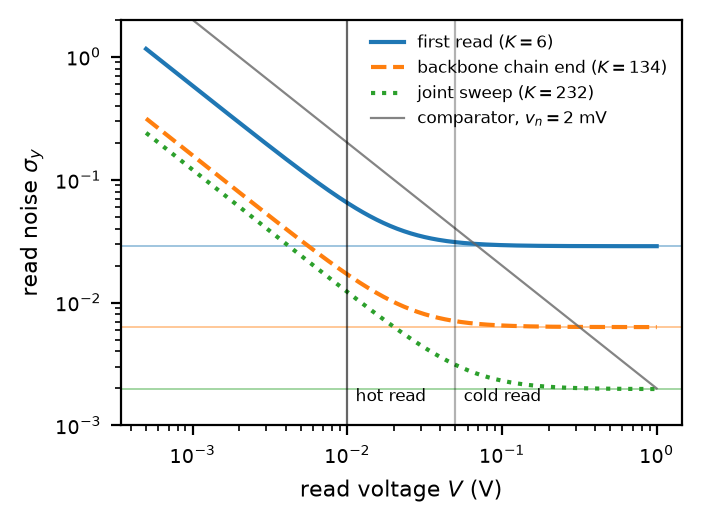
\includegraphics[width=\columnwidth]{figures/fig-noise.png}
\caption{\textbf{The devices alone set only the floor of a read's
noise, and pooling lowers that floor.} Read noise against read
voltage at the settling-limited pulse of Sec.~\ref{sec:comparator}.
The thermal term is the kT/C noise of the lane's output node, from
the geometry of Appendix~\ref{app:energy} plus 5\,fF of comparator
input, for the first read of the chain ($K = 6$), the end of the
backbone chain ($K = 134$), and the joint sweep ($K = 232$); the thin
horizontal lines are the flicker floors at each pool's measured
magnitude. Node capacitance grows with the number of pooled pairs, reducing
noise by up to a factor of five relative to the first read. The comparator's operating level, $v_n = 2$\,mV, is
drawn for scale: at the 10\,mV hot read it is the larger term on
every read.}
\label{fig:noise}
\end{figure}

\subsection{The neural lane}\label{sec:lane}

A neural lane is an array of unit-crossbar pairs pooled on a shared
2-1 divider. By Kirchhoff's laws the selected pairs report
\begin{equation}
y = \frac{\sum_{i \in \mathcal{A}} (G_{a,i} - G_{b,i})}
         {\sum_{i \in \mathcal{A}} (G_{a,i} + G_{b,i})}
  = \frac{\sum_{i \in \mathcal{A}} m_i w_i}
         {\sum_{i \in \mathcal{A}} m_i},
\label{eq:pool}
\end{equation}
the magnitude-weighted average of the selected weights. Selection is an
Activation Address Tuple (AAT): an ordered tuple of integers, one per
address space. Each space influences a read in proportion to its share of the pooled
magnitude, roughly $1/K$ for $K$ active spaces. Addresses without
measured values therefore dilute those with measured values.
Conditioning addresses must be repeated across several spaces to have
enough influence. These constraints determine the model class.

Instruction codes in the kT-RAM instruction set (Table~\ref{tab:isa})
are two letters: the first is the drive direction (F forward, R
reverse), the second the operation. Forward feedback accumulates
magnitude and reverse feedback depletes it; every working routine
pairs a forward operation with a reverse one.

\begin{table}
\caption{The kT-RAM instruction set. \label{tab:isa}}
\begin{ruledtabular}
\footnotesize
\begin{tabular}{p{1.75cm}p{2.1cm}p{3.6cm}}
Instruction & Kind & Effect \\
\colrule
\texttt{FF}, \texttt{RF} & read, full voltage & return $y$; the drive
adapts the pair (repeated \texttt{FF} anti-Hebbian, \texttt{RF}
Hebbian) \\
\texttt{FFLV}, \texttt{RFLV} & read, subthreshold & return $y$ with
zero disturbance \\
\texttt{FH}/\texttt{RH}, \texttt{FL}/\texttt{RL} & supervised
feedback & drive $w$ up / down \\
\texttt{FU}/\texttt{RU}, \texttt{FA}/\texttt{RA} & unsupervised
feedback & reinforce / oppose the current sign \\
\texttt{FZ}, \texttt{RZ} & zero feedback & no push on $w$; $m$ grows
/ shrinks \\
\end{tabular}
\end{ruledtabular}
\end{table}

\subsection{WTA Groups and the lane routines}\label{sec:routines}

Lanes form winner-take-all (WTA) Groups, with one lane per address-space
symbol. This paper uses three routines, described in detail in an online
chapter series \cite{knowm2026blog}. In the \emph{supervised three-case rule}, all
lanes of a group are read with \texttt{FF}; the labeled lane receives
\texttt{RH}; a wrong lane that fired receives \texttt{RL} (hard) or
nothing beyond the paired reverse read (soft); a correctly silent lane
receives \texttt{RF}. Cold argmax readout of a group taught this way
is a classifier at parity with logistic regression on the identical
encoding (Iris: 0.962 against 0.961 over twenty splits). Hard feedback creates a margin between the winner and the other lanes.
Soft feedback retains all outcomes supported by the data, so a hot read
samples from a distribution defined by the learned lane scores. Generation runs as sequential lane reads: clamp
what is known, read one space, commit, continue. \emph{RankCut} ranks a group's above-threshold lanes using a shared
falling reference and one comparator per lane. It requires no per-lane
analog-to-digital converter. 

\subsection{The emulator}\label{sec:emulator}

All results are emulated lane computation on
\texttt{ktram-neural-core} \cite{knowm2026emulator}: device models
with the read-noise physics above, a torch runtime bit-exact against
the reference core, and every read and adapt issued as a lane
instruction. The emulator's crossbar fidelity is ideal: a read returns
the selected pair of each space alone, with no contribution from the
unselected devices of the unit crossbar
(Limitation~\ref{lim:sneak}). The physical memristors and crossbars
exist as fabricated and commercially sold hardware
\cite{knowm2026datasheet}; the lane-scale system does not yet. The emulator's device noise gain stays fixed at its reference value of
0.02, including during hot reads. A hot read is driven by the read voltage
and by the comparator term of Eq.~(\ref{eq:noise}), both physical
operating points.

\section{The model class}\label{sec:model}

\subsection{The code}\label{sec:code}

We encode images with per-position dropout additive quantization
(dropout-AQ): $k$ books of $S$ atoms, with keep probability $p$. This
approach builds on vector and additive quantization
\cite{gray1984vq,jegou2011product,babenko2014additive} and on generation
from discrete codes \cite{vandenoord2017vqvae,chang2022maskgit}. A code is a point in
$\A_S^k$ ($k$ address spaces of $S$ symbols each), mirroring the
codeword space $\mathbb{F}_q^n$ of coding theory. The training
objective marginalizes Bernoulli address deletion,
\begin{align}
\mathbb{E}_z \Bigl\| x - b - \sum_j z_j a_j \Bigr\|^2
&= \Bigl\| x - b - p \sum_j a_j \Bigr\|^2 \nonumber \\
&\quad + p(1-p) \sum_j \| a_j \|^2,
\label{eq:dropoutaq}
\end{align}
with $z_j \sim \mathrm{Bernoulli}(p)$. Both partial and complete codes
use the same fixed linear decoder:
\begin{equation}
\hat{x} = b + p \sum_{j \in \mathrm{present}} a_j .
\label{eq:decode}
\end{equation}
The codebooks are fitted on the host by alternating discrete encoding
and a joint double-precision ridge solve. At $p=1$, the objective is standard additive quantization
\cite{babenko2014additive}. At $p<1$, training also includes partial
codes, though some may still decode to incoherent images.

Stripped of the hardware, the model class is generation over a linear
additive-quantization codebook with masked-context training and a
parallel reconciliation sweep, which places it beside MaskGIT
\cite{chang2022maskgit} and the VQ-VAE lineage
\cite{vandenoord2017vqvae}. The fixed linear decoder handles partial codes and can run as lane
reads, whose energy is counted in Sec.~\ref{sec:energy}. Each level pairs a soft bank for sampling with a hard bank for repair,
both trained through local lane instructions. A masked transformer uses
one network and a confidence schedule.

\subsection{Paired banks and the generation procedure}\label{sec:banks}

Each CHILL ZEN level pairs a soft generator bank G with a hard repair
bank R. G uses hot reads. R trains on corrupted pools and uses one cold
parallel sweep to commit all updates. The two-level system evaluated here has a
\emph{backbone} (level 1: a global code over the whole canvas, with
banks G1 and R1) and a \emph{patch level} (level 2: a residual code on
a grid of patch slots, with bank G2 and a cross-level joint repair
bank). The \emph{render} is the backbone decode plus the patch decode.
For context $c=(z_{<m},\ell)$, the draw is
\begin{equation}
 z_m = \arg\max_s\{y_{m,s}(c)+\epsilon_{m,s}\},
 \qquad \epsilon_{m,s}\sim\mathcal{N}(0,\sigma_{m,s}^2),
\end{equation}
with independent noise in the emulator. This defines a conditional
choice probability for each symbol; the teaching rule does not
calibrate it to the data conditional. Generation runs as follows
(Fig.~\ref{fig:arch}):

\begin{enumerate}
\item Clamp the label, replicated across six address spaces.
\item Backbone draw: read the 128 global books autoregressively,
  choosing the lane with the highest noise-perturbed score at each step,
  then apply one cold R1 sweep. Hot reads use $(V, v_n) =
  (10\,\mathrm{mV}, 2\,\mathrm{mV})$, the best critic setting on the
  tested grid (Sec.~\ref{sec:comparator}). Section~\ref{sec:headtohead}
  reports FID at its own best setting on that grid.
\item Patch level: one parallel hot G2 read, at the same operating
  point, over all 49 residual patch slots under the held global code.
\item One cold cross-level joint sweep reconciles both levels: all
  226 addresses are targets, and the sweep may flip globals bottom-up
  and patches top-down in the same parallel read.
\item Decode and render: the fixed linear map of Eq.~(\ref{eq:decode}),
  run in host floating point in this paper's emulation and counted in
  Sec.~\ref{sec:energy} as the lane read it is designed to be.
\end{enumerate}

Generation takes 131 sequential steps per image: 128 autoregressive
reads and three parallel sweeps. Running the step 5 decoder on lanes
adds one parallel read. The
temperature schedule has two values. Every
read uses the same read voltage, so the temperature is the
comparator's noise setting alone: $v_n = 2$\,mV for draws and
$v_n \to 0$ for decisions. Both settings occur within one image.
% 37_dose_chain.py (and --quench): the sweep chained to eight doses.
The joint sweep runs once by design, because repeating it degrades
the image. Each further cold dose lowers the critic by about 0.01,
from 0.90 after one dose to 0.81 after eight, and pulls diversity and
tone toward the class prototypes. Real encoded codes drift the same
way under repeated doses. The sweep's fixed points are the class
prototypes, and the data are not among them.
Warming the sweep does not help. With read noise at a
tenth of the read voltage the critic stops decaying over doses and
holds near 0.85, but diversity still falls, from 0.63 to 0.56 by the
eighth dose. At the draw's own operating point the sweep no longer
functions: it flips about 200 of the 226 addresses on every dose and
the critic drops below 0.5 after the first.

\begin{figure}
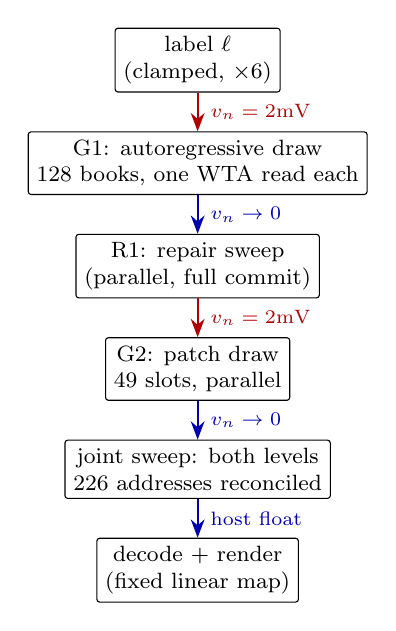
\begin{tikzpicture}[
  font=\footnotesize,
  box/.style={draw, rounded corners=1pt, align=center,
              inner sep=3pt, minimum height=18pt},
  hot/.style={-{Stealth}, thick, red!70!black},
  cold/.style={-{Stealth}, thick, blue!70!black},
  lbl/.style={font=\scriptsize, midway, right=1pt}]
\node[box] (label) {label $\ell$\\(clamped, $\times 6$)};
\node[box, below=14pt of label] (g1) {G1: autoregressive draw\\128
  books, one WTA read each};
\node[box, below=14pt of g1] (r1) {R1: repair sweep\\(parallel,
  full commit)};
\node[box, below=14pt of r1] (g2) {G2: patch draw\\49 slots,
  parallel};
\node[box, below=14pt of g2] (joint) {joint sweep: both levels\\226
  addresses reconciled};
\node[box, below=14pt of joint] (render) {decode + render\\(fixed
  linear map)};
\draw[hot] (label) -- (g1) node[lbl] {$v_n = 2$mV};
\draw[cold] (g1) -- (r1) node[lbl] {$v_n \to 0$};
\draw[hot] (r1) -- (g2) node[lbl] {$v_n = 2$mV};
\draw[cold] (g2) -- (joint) node[lbl] {$v_n \to 0$};
\draw[cold] (joint) -- (render) node[lbl] {host float};
\end{tikzpicture}
\caption{\textbf{One CHILL ZEN generation uses both temperature
regimes in turn.} Hot reads (red) draw the code and cold sweeps (blue)
reconcile it; exactly two arrows are hot, both at the operating point
$(V, v_n) = (10\,\mathrm{mV}, 2\,\mathrm{mV})$ of
Sec.~\ref{sec:comparator}.}
\label{fig:arch}
\end{figure}

\section{Training and results}\label{sec:results}

\subsection{Setup and metrics}\label{sec:setup}

The benchmark is grayscale Fashion-MNIST \cite{xiao2017fashion},
split 68\,000 train and 2\,000 evaluation. We report four metrics. \emph{Critic} measures label agreement using a
frozen pixel-space multilayer perceptron
($784\to256\to\mathrm{ReLU}\to10$); the target is its score on real
images. \emph{Div} measures within-class diversity as the fraction of
pixel pairs differing by more than $1/16$. \emph{Tone} measures the
within-class spread of each image's mean foreground level.
\emph{Std-ratio} measures foreground contrast relative to real images,
with an alarm threshold of 1.10. Section~\ref{sec:headtohead} reports FID on binarized renders using
the DTM replication protocol.

The banks are trained using local lane instructions without gradients. The
codec is fitted on the host, and the frozen critic is trained with Adam. Soft G banks train on Bernoulli-masked codes with labels retained. Hard
R banks train on pools corrupted by marginal sampling and G fills. The
joint bank trains on corrupted two-level states. Each bank is probed per epoch on the same 2000-image evaluation
partition and the best-probe snapshot is kept. That partition also
informed the fill-noise and generation-noise choices; it is a
validation set, not an untouched test set. New generation seeds
measure sampling variation for the selected banks, not uncertainty
from training or model selection.

Repair-training fills use the 10\,mV read with comparator register
code 245 ($v_n=5$\,mV). This setting was chosen during development
and carried over to the binary-trained stack. These runs cannot isolate the effect of fill noise: generation noise
also varied, and the intermediate fill-sweep logs were not retained. The released scripts reproduce the final recipe.
Two choices in that recipe, holding the label and committing a single
cold dose, follow the pool-share argument of Sec.~\ref{sec:lane}.

\subsection{The two-level result}\label{sec:headline}

The deployed system is a 904-bit code plus the clamped label: a
$128\times16$ global backbone at keep-$p$ 0.5 (512 bits) and a
$2\times16$ residual patch code on a $7\times7$ grid of
$4\times4$-pixel slots (392 bits). Table~\ref{tab:headline} reports means and seed ranges (max $-$ min)
over three generation seeds at $n=1000$, with one fitted set of banks.
The reconstruction arm supplies a real backbone code directly to G2,
bypassing both the autoregressive draw and R1; G2 and the joint sweep
then run as deployed. It tests those downstream stages together,
rather than isolating the draw alone.

The reconstruction and end-to-end critic scores are 0.8963 and 0.9007,
against 0.8860 for the first 100 validation images per class. These
are label-agreement scores, not evidence that generated images match
or exceed real-image quality. A classifier can score class
prototypes highly. End-to-end tone variation is lower than real (1.590
against 2.362), while contrast is higher (1.14 against 1.00) and
exceeds the stated 1.10 alarm. The seed ranges are descriptive;
they are not confidence intervals or a test of equivalence.

% Both rows: 21_reporting.py, both arms with their hot reads at the
% operating point (V, v_n) = (10 mV, 2 mV), seeds 960-962.
\begin{table}
\caption{The two-level model scored: mean (seed range, max $-$ min)
over three generation seeds at $n = 1000$. Both arms run their hot reads at the
operating point of Sec.~\ref{sec:comparator}; the reconstruction arm bypasses the draw and R1 with a real backbone
code; the end-to-end arm draws from the label alone.
\label{tab:headline}}
\begin{ruledtabular}
\footnotesize
\begin{tabular}{lcccc}
arm & critic & div & tone & std-ratio \\
\colrule
real references & 0.8860 & 0.4866 & 2.362 & 1.00 \\
reconstruction & $0.8963\ (0.0110)$ & $0.5184\ (0.0015)$
  & 2.004 & 1.13 \\
end-to-end & $0.9007\ (0.0310)$ & $0.5487\ (0.0052)$ & 1.590
  & 1.14 \\
\end{tabular}
\end{ruledtabular}
\end{table}

\begin{figure*}
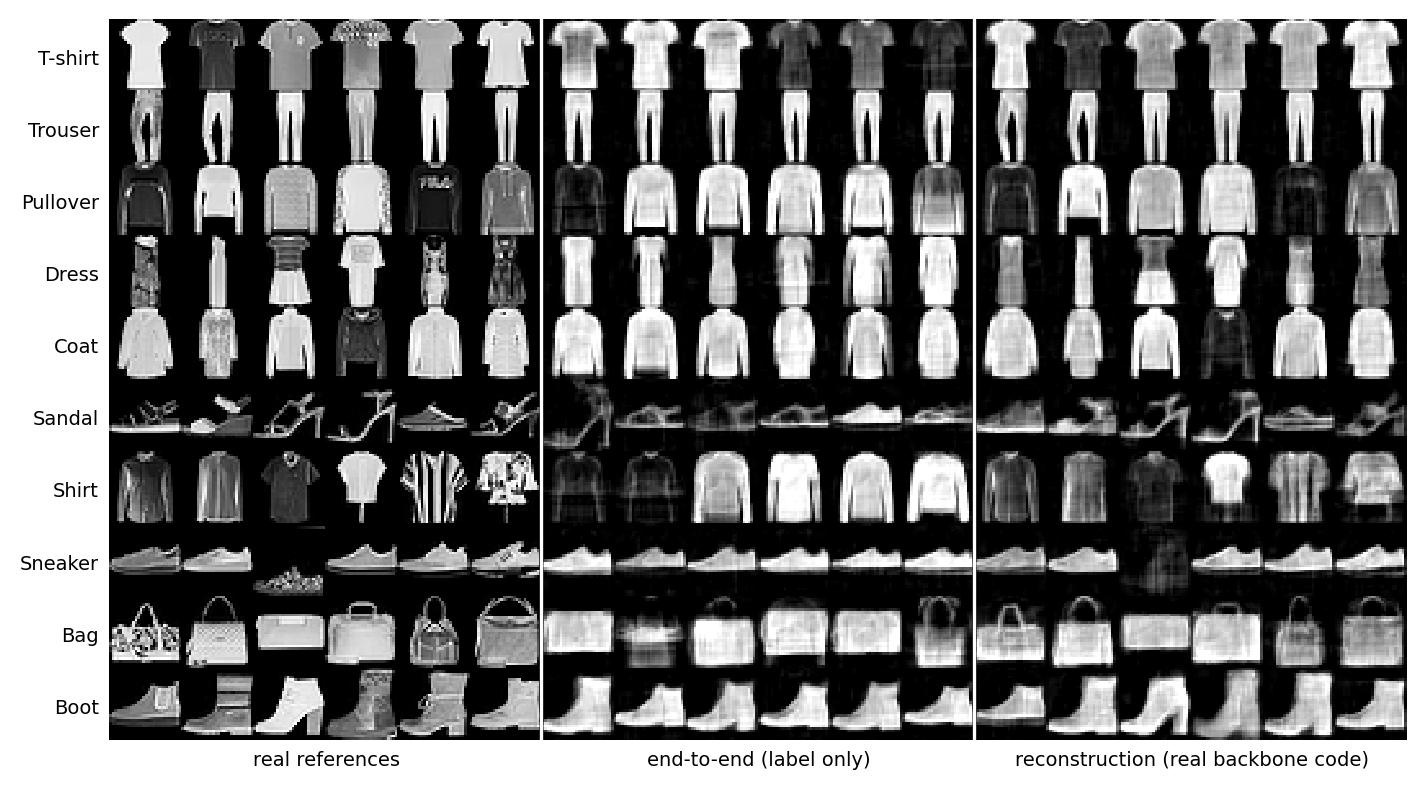
\includegraphics[width=\textwidth]{figures/fig-samples.png}
\caption{\textbf{Given a real backbone code, the patch level and joint
sweep produce images with similar classifier agreement to real ones.} Real
references (left), end-to-end draws from the label alone at the
operating point of Sec.~\ref{sec:comparator} (center), and the
reconstruction arm (right), six per class. The strips are the first six samples per
class from reporting seed 960 ($n=1000$), with no sample selection.}
\label{fig:samples}
\end{figure*}

% Memorization: 21_reporting.py. Stack arms at n = 320: 08_stack_arms.py.
The generated batch shows no memorization signature: over 5120 drawn
images every joint and backbone code is distinct, none is an exact
copy of a training image, and their nearest-neighbour distances to the
training set sit at or beyond those of held-out real images ($L_2$
first percentile 1.86 against 1.47, median 3.70 against 3.43).
The code still changes after one joint sweep: the second sweep changes
82 of 226 addresses per image, the third 44, and the fourth 26.

\subsection{The comparator sets the draw temperature}\label{sec:comparator}

Every hot read in this paper runs at a modeled read voltage of
$V = 10$\,mV, with the pulse width settling-limited,
$t_b = \max(2\,\mathrm{ns}, 5RC)$. We assume a minimum read voltage of 10\,mV, called the sense floor. At
this voltage, the target 1\,mV trimmed comparator offset is 10\% of full
scale (Sec.~\ref{sec:ktbit}). Kickback is a separate, unresolved
readout requirement (Appendix~\ref{app:energy}). At this voltage, the model gives device read noise of 0.02--0.04 across
the backbone chain. Flicker accounts for 70\% of the variance on the
first read, when only the replicated label is present. Its share falls
to 5\% by the last read, where thermal noise dominates. The model's thermal noise stays nearly constant along the chain.
Settling time cancels the conductance dependence, leaving the kT/C term
of Sec.~\ref{sec:ktbit} with node capacitance fixed at 100\,fF. The geometry of Appendix~\ref{app:energy} puts the node
at about 12\,fF on the first read and 161--278\,fF thereafter, so by
that geometry the first read is noisier than modeled, about 0.07, and
the later reads are as modeled. At this voltage, the lanes supply less than 40\% of the required draw
noise on the first read and less than 10\% thereafter. Their thermal
contribution is set by the node's kT/C noise. Supplying enough noise
from the node alone would require a read voltage near 1\,mV. Circuit settings can increase the comparator term $v_n / V$ in
Eq.~(\ref{eq:noise}), which is independent of $y$ and $m$
(Table~\ref{tab:comparator}).

\begin{table}
\caption{Comparator design classes and the numbers this paper models
against: kT/C plus preamplifier thermal noise, referred to the input;
offset from transistor mismatch \cite{pelgrom1989matching}. The last
column refers the offset to the 10\,mV hot read, where a lane's
output spans $\pm 1$. A digital trim removes offset and leaves the
noise of the underlying class.
\label{tab:comparator}}
\begin{ruledtabular}
\footnotesize
\begin{tabular}{lccc}
class & noise (rms) & offset & offset / 10\,mV \\
\colrule
raw dynamic latch & 0.5--2\,mV & 5--20\,mV & 0.5--2 \\
auto-zeroed / chopped & 50--200\,$\mu$V & 0.1--1\,mV & 0.01--0.1 \\
either, trimmed & as above & tens of $\mu$V & $\sim 0.003$ \\
\end{tabular}
\end{ruledtabular}
\end{table}

\emph{The sweep.} We swept $v_n / V$ at $V = 10$\,mV from 0 (lanes
only) to 0.20 on the grayscale end-to-end draw and to 0.50 on the
binary-trained two-level draw of Sec.~\ref{sec:headtohead}, holding
every other component as deployed. Both stacks improve with added comparator noise (Fig.~\ref{fig:comparatorsweep}): the best grayscale critic occurs at the tested endpoint $v_n / V=0.20$, and binary FID is lowest at $0.2$--$0.3$. The binary optimum lies on two grid points added after a first pass. A 7.5\,mV point tested before the register was introduced exceeds its ceiling and is not reported.

The comparator-noise level is a tunable model parameter. The emulator sets comparator noise with an 8-bit trim register: $v_n =
100\,\mu\mathrm{V} + \mathrm{code} \times 20\,\mu\mathrm{V}$ for codes
0--255. We report noise levels by code. The full test grid uses codes 3,
20, 45, 95, 145, and 245. The grayscale critic sweep uses the first
four; the grayscale FID sweep uses the first five plus a device-only
point (Sec.~\ref{sec:headtohead}). No comparator has zero input-referred noise, so the register has no
zero-noise setting. We use $v_n / V = 0$ only to model device noise
alone. At $V = 10$\,mV
the register's ceiling of 5.20\,mV caps $v_n / V$ at 0.52, which is
where the sweep stops.

% Sweep: 23_comparator_sweep.py, 24_binary_comparator_sweep.py.
At the optima the comparator
supplies 97--99\% of the read's variance in the grayscale draw and
99--100\% in the binary one as modeled; at the first read's node
capacitance of Appendix~\ref{app:energy} the grayscale share on that
read is about 90\%. At fixed $v_n / V = 0.10$, raising the read voltage from 10 to 50\,mV
reduces lane thermal noise fivefold with little change in the metrics:
grayscale critic 0.8837 versus 0.8840 and binary FID 10.73 versus 10.99.
This supports comparator noise as the main control of sampling
temperature. The two terms also differ along
the chain. Device noise falls as $1/\sqrt{m}$, making it greatest early in the
chain, when the pool is small, and least at the end. Comparator noise
stays constant along the chain.

\begin{figure}
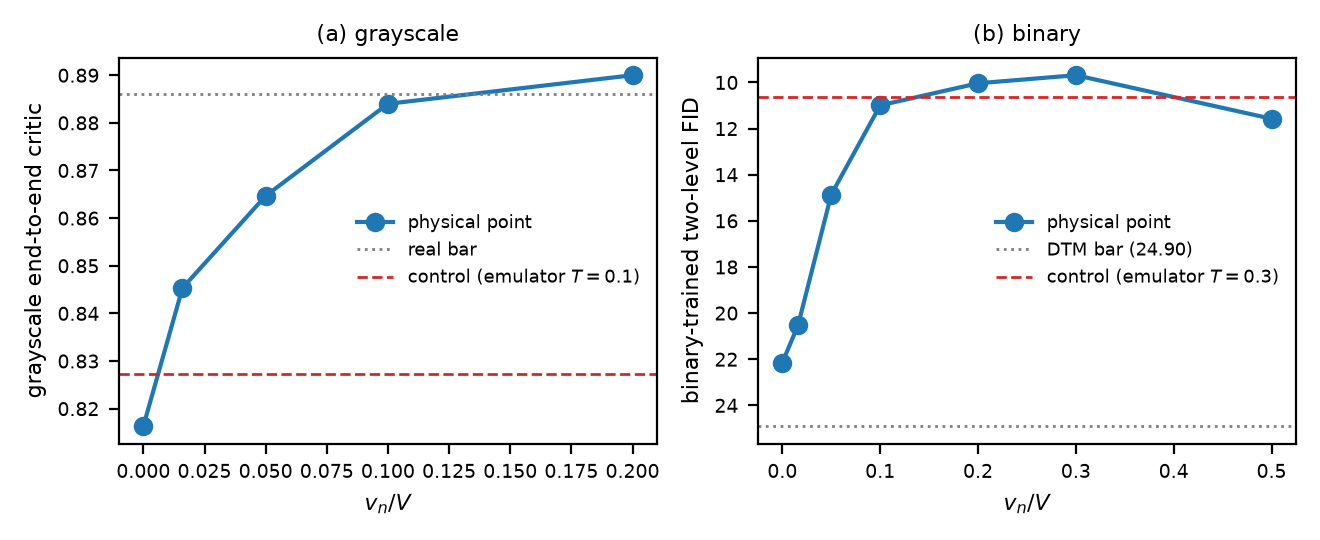
\includegraphics[width=\columnwidth]{figures/fig-comparator-sweep.png}
\caption{\textbf{The comparator's noise setting is the draw
temperature.} (a) The grayscale end-to-end critic against the
comparator's input-referred noise relative to the read voltage, at
$V = 10$\,mV, with the real bar drawn as a line. (b) The same sweep
on the binary-trained two-level stack, scored as FID under the
protocol of Sec.~\ref{sec:headtohead}, with the DTM reference arm's
FID drawn as a line.}
\label{fig:comparatorsweep}
\end{figure}

\emph{The design requirement.} No comparator class reaches these
operating points on its own. At a 10\,mV read, a dynamic latch's own kT/C and preamplifier noise can
reach $v_n / V \approx 0.2$ with low preamplifier bias. This reaches the
grayscale optimum of 0.20. The binary optimum of 0.2--0.3 may require
still lower bias or an added input noise source. But the same latch carries
5--20\,mV of offset, which at a 10\,mV read is 0.5--2 of the full
range of a lane's output (Table~\ref{tab:comparator}), and no shift of
the weights cancels an offset larger than the range. Static offset and read noise require separate control mechanisms. CHILL ZEN requires comparator offset below about 10\% of the read
voltage at every operating bias: 1\,mV at a 10\,mV read. Each lane needs
a one-time trim if its offset exceeds this limit. Input-referred noise
must be adjustable from near zero to about 20--30\% of the read voltage,
using reduced preamplifier bias or an added noise source. A higher hot-read voltage allows more offset if $v_n / V$ stays fixed,
as the 50\,mV test above supports. At 50\,mV, the allowed offset
increases fivefold, but a hot read at $v_n / V = 0.20$ needs 10\,mV rms
of comparator noise.

% Cold-read control: 35_cold_noise_control.py.
\emph{The cold reads.} The deployed generation runs its two cold
sweeps at zero read noise. A physical cold read has a floor: at
50\,mV the combined noise comes to about 0.003 of the read. To
measure what that floor does, we ran both sweeps at zero noise, at
the floor, and at ten times the floor, on the same hot draws, three
seeds at $n = 1000$. The noise flips decisions, 9 of the 128 R1 addresses and
12 of the 226 joint addresses per image at the floor, and a quarter of
the R1 addresses and 52 of the joint addresses at ten times it. The
metrics do not move: critic 0.890 against 0.890 at the floor and
$0.893 \pm 0.024$ against $0.890 \pm 0.012$ at ten times it, with
diversity, tone, and contrast unchanged. The aggregate metrics show no detectable effect of replacing noiseless
cold reads ($T=0$) with the physical noise floor. We did not repeat the
comparison in Sec.~\ref{sec:headtohead} with that floor applied. Appendix~\ref{app:energy} gives conditional noise-energy
estimates; the bandwidth, noise, and energy have not been demonstrated
together in one comparator.

\subsection{What the controls establish}\label{sec:gap}

The reconstruction arm feeds real backbone codes to G2 and the joint
sweep, and the critic holds. This test checks those two banks but does not locate the source of the
final tone and contrast errors. It skips the draw and R1, and its
classifier score does not fully describe the image distribution. The reconstruction FIDs of Sec.~\ref{sec:headtohead}
are likewise a reference for the code, not a bound on a generator.

At the operating point in Sec.~\ref{sec:comparator}, comparator noise is
fixed at $v_n / V = 0.20$ for every draw read. Contrast nearly matches
the reconstruction arm (std-ratio 1.14 versus 1.13), while tone spread
is lower (1.59 versus 2.00; Table~\ref{tab:headline}).

\subsection{Design studies}\label{sec:studies}

Two scaling studies set the deployed code, both measured on the
pipeline this paper describes.

\emph{(a) Capacity and alphabet scaling.} At fixed alphabet size and keep probability $p=0.5$, increasing from 64
to 128 books raised the backbone-only critic score from 0.813 to 0.834.
The larger-alphabet configuration scored lower: 0.7875 for $64\times32$
at 320 bits versus 0.8344 for $128\times16$ at 512 bits. Both alphabet
size and bit count changed in this comparison. A global code
removes tile seams by construction: the mean pixel step across tile
boundaries, relative to elsewhere, is 0.93--1.07 for the global code
with real images at 1.100 (Fig.~\ref{fig:backbone}).

\emph{(b) Codec rate--distortion.} At 512 bits, the global dropout-AQ code achieves its lowest relMSE,
0.0500, at keep probability $p=0.75$. The deployed $p=0.5$ code has
relMSE 0.0612 but greater cross-address coherence, as described below.
The two-level residual code reaches relMSE 0.0382
(Fig.~\ref{fig:codec}). As plain additive quantization ($p = 1$) scales up, unused atoms and
stalled search reduce its accuracy. The lowest reconstruction error
occurs at $p = 0.75$. Using $p = 0.5$ raises that error by 12--22\% but
provides 2.2--3.6 times the cross-address coherence needed for
generation. Both increases are largest at 128 books.

\begin{figure}
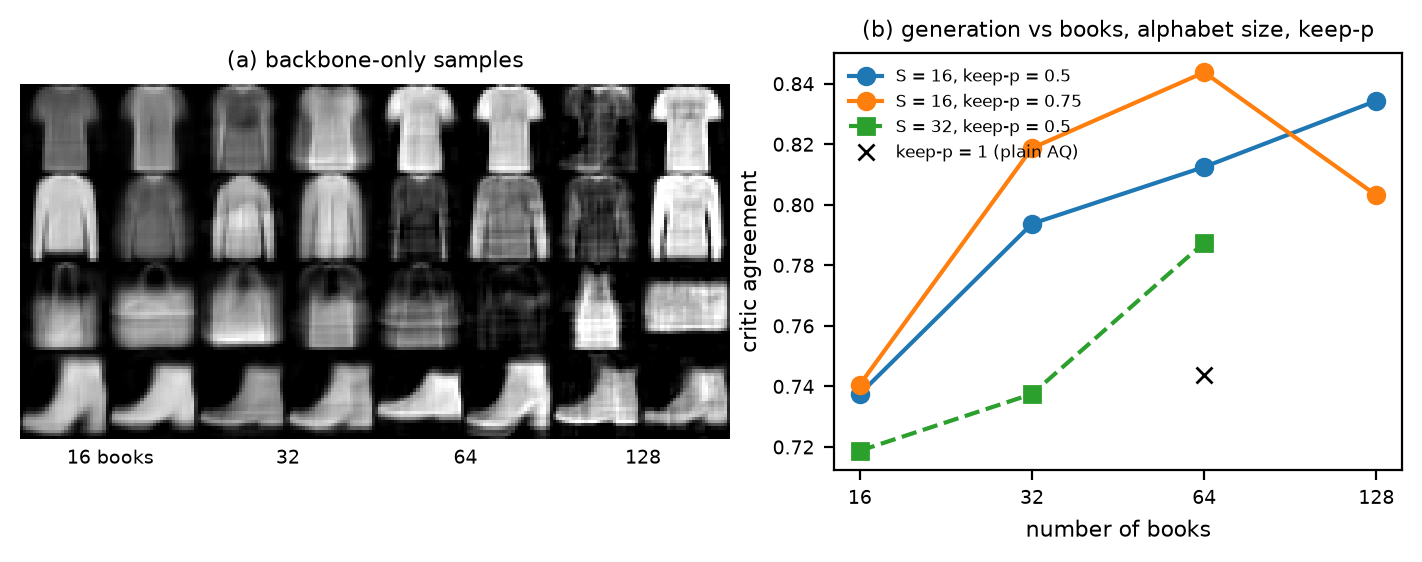
\includegraphics[width=\columnwidth]{figures/fig-backbone.png}
\caption{\textbf{A single additive code over the whole canvas has no
patch seams and improves with the number of books at fixed alphabet.}
(a) Backbone-only samples at 16, 32, 64, and 128 books. (b) Critic
agreement against the number of books and the alphabet size: the larger-alphabet configuration scored worse, but its lower bit count
prevents attributing the difference to alphabet size alone. Plain
additive quantization ($p = 1$) underperforms the dropout code.}
\label{fig:backbone}
\end{figure}

\begin{figure}
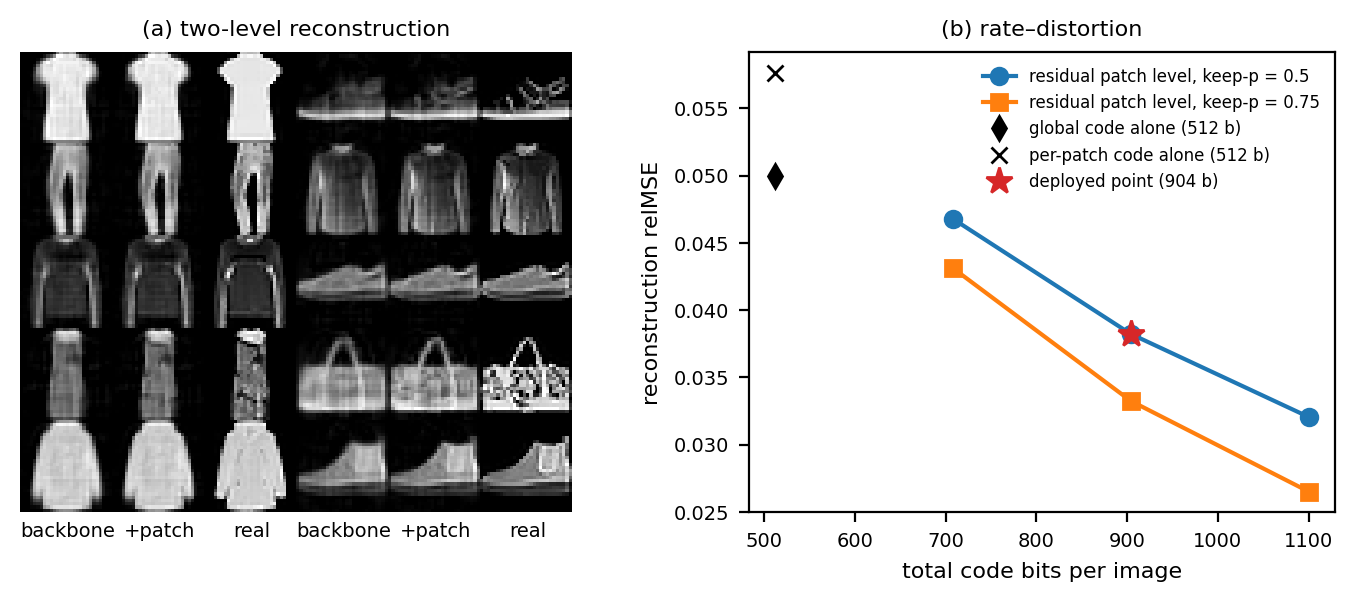
\includegraphics[width=\columnwidth]{figures/fig-codec.png}
\caption{\textbf{The residual construction reaches the program's
lowest reconstruction floor.} (a) Backbone decode, backbone plus patch
decode, and the real image, one example per class. (b)
Rate--distortion of the residual patch level over the 512-bit global
backbone; the deployed 904-bit point reaches relMSE 0.0382, and the
global code alone outscores a per-patch code at rate parity.}
\label{fig:codec}
\end{figure}

\section{Comparison with the DTM/DTCA}\label{sec:comparison}

\subsection{The design points}\label{sec:designpoint}

The two systems differ as design points (Table~\ref{tab:designpoint});
our reading of the DTM/DTCA follows
Ref.~\cite{jelincic2025dtm} and its released software
\cite{extropic2025thrml}.

\begin{table*}
\caption{Two thermodynamic design points. Claims in the left column
are from Ref.~\cite{jelincic2025dtm}. \label{tab:designpoint}}
\begin{ruledtabular}
\begin{tabular}{p{2.9cm}p{6.9cm}p{6.6cm}}
 & DTM / DTCA \cite{jelincic2025dtm} & CHILL ZEN (this work) \\
\colrule
generative principle & reverse a noising chain; each step an EBM
sampled by Gibbs & draw an address code hot; one cold repair sweep
reconciles \\
sampling procedure & $K_{\mathrm{mix}} = 250$ Gibbs iterations per
step, $T = 2$--$8$ steps & 128 autoregressive reads + 3 parallel
sweeps $\approx$ 131 sequential steps \\
random draws per image & $T K L^2 \approx 8 \times 250 \times 4900
\approx 10^{7}$ conditional updates & about 3600 hot lane reads \\
randomness source & dedicated subthreshold-transistor RNG,
free-running, $\tau_0 \approx 100$\,ns & one comparator per lane, its
input-referred noise settable; the pooled weights' own
read noise is the minor term \\
temperature control & $\tau_0$ fixed by circuit design & the read
voltage and the comparator's noise setting; cold reads are
modeled as noiseless \\
noise character & bias-programmable Bernoulli source & a flat settable
term from the comparator, plus a state-dependent device term that
pooling quenches \\
weights and sampler & separate circuit elements (couplings; RNG
nodes) & the stored weight, read through one comparator per lane that
is also the sampler \\
data representation & binarized Fashion-MNIST, $\pm1$ spins &
grayscale Fashion-MNIST, 904-bit address code; binarized host-side
for Sec.~\ref{sec:headtohead} \\
rendered output & binary spins; grayscale via a multi-spin embedding;
color via a GAN-tuned neural decoder & float grayscale via a fixed
linear decode \\
learning & Monte Carlo gradient estimates from equilibrium samples
(host optimizer) & local lane instructions for banks; host-fitted
codebooks \\
\end{tabular}
\end{ruledtabular}
\end{table*}


The DTM chain keeps each step easy to mix, but its sampling cost still
depends on the number of steps and iterations. CHILL ZEN has no mixing
phase, so we report no mixing time. The remaining challenge is the
quality of its draws. Both systems obtain their randomness
from a circuit at each node, and what separates them is how many draws
an image needs, about 3600 hot lane reads against about $10^{7}$
conditional updates at their stated $K_{\mathrm{mix}} = 250$. The systems do different amounts of work per step, so step counts alone
cannot compare their energy use. We therefore estimate energy in joules;
neither system has been fabricated at the target scale.

\subsection{Energy}\label{sec:energy}

% 12_energy_model.py, 13_energy_frontier.py, 22_binary_energy.py;
% Fig. 9: 15_energy_figure.py. The model is chill_zen/energy_geom.py;
% Appendix B gives every number behind this section.
For a read whose noise is thermally limited, the referred noise and
the dissipation are
\begin{equation}
\sigma^2 = \frac{2 \kB T}{t V^2 G_\Sigma}, \qquad
E = V^2 G_\Sigma t,
\end{equation}
where $G_\Sigma$ is the selected-pool conductance and $t$ the read
pulse width, and their product eliminates the device entirely:
\begin{equation}
E_{\mathrm{read}} \, \sigma^2 = 2 \kB T .
\label{eq:ethermal}
\end{equation}
The energy of one stochastic sample at noise level $\sigma$ is set by
thermodynamics alone, for a pooled lane read exactly as for a single
device. For a comparator that samples the node at settling-limited
timing the realized product is $5 \kB T$ (Appendix~\ref{app:energy}).
The identity covers only the lane's noise contribution, with an energy
cost of roughly $10^3$--$10^4\,\kB T$ per read at the deployed noise
levels. The lane supplies just 1--3\% of the draw's variance at the
operating point in Sec.~\ref{sec:comparator}. The comparator supplies the remaining noise at about 10\,fJ per lane
read, or roughly $10^6\,\kB T$. A DTCA draw costs less: its RNG uses a
measured 350\,aJ per bit, and a full cell update uses about 2\,fJ,
including the RNG, bias, clock, and communication
\cite{jelincic2025dtm}. The identity sets the energy of only the smaller noise contribution and
is not used in the estimates below. Total energy also depends on how
many draws each system needs: the accounting below counts about 3600
noisy reads per image, where the chain counts $T K L^2 \approx 10^{7}$
conditional updates.

The per-image energy is a conditional estimate from the stated geometry
of Appendix~\ref{app:energy}: the neural lane of
Ref.~\cite{knowm2026blog}, one $4 \times 4$ unit-crossbar pair per
address space on a 50\,nm pitch, the address of a read broadcast on
select lines across every lane of a bank, and the unselected lines
floating (Limitation~\ref{lim:sneak}). The model counts three energy terms per image: address delivery at the
select supply, $E_{\mathrm{sel}}$; divider reads at
$5\,C_{\mathrm{node}} V^2$ each, independent of device conductance,
$E_{\mathrm{read}}$; and one comparator and lane buffer per lane read,
$E_{\mathrm{readout}}$. Readout assumes a continuous-time comparator;
Table~\ref{tab:readout} gives alternatives. Rail energy is below
$10^{-11}$\,J and is omitted. It is applied to the exact operation count of the
deployed system, 10\,064 lane reads and $1.78\times10^{6}$ address
assertions over five banks totalling about $2.9\times10^{7}$ synapse
pairs, with constants that are each a stated dimension or a textbook
value (Table~\ref{tab:app-constants}).  The decoder is the fixed linear map of Eq.~(\ref{eq:decode}): with the codebook atoms stored as differential
pairs, one output lane per pixel, and every code address present at
the end of a generation, the pooled read of Eq.~(\ref{eq:pool})
returns the sum of the selected atoms at a fixed scale. Decoding
accounts for about 8\% of all reads. This paper's emulation runs that map in host
floating point, as it does the render and the judging; the model
counts it as the 784 cold lane reads it is designed to be. Running it
on lanes, with the atoms quantized to a pair's resolution and read at
50\,mV, has not been emulated and its precision is not measured. The
DTM has no decode for binarized Fashion-MNIST because its spins are
the pixels. This saving applies to binary pixels. The DTM uses a multi-spin
embedding for grayscale and a separately trained neural decoder for
color (Table~\ref{tab:designpoint}), both excluded from its energy
estimate. Our Sec.~\ref{sec:results} system generates grayscale images,
which we binarize for the comparison. The model's address-delivery term is
what Ref.~\cite{jelincic2025dtm} calls $E_{\mathrm{comm}}$ and
reports as about half of its budget.

Address delivery is 91\% of the total at the nominal point, readout
8\%, and the divider reads 1\%. Table~\ref{tab:energy} reports the nominal energy estimate and its
sensitivity to the select supply and peripheral circuit design rules.
\begin{table}
\caption{Modeled energy per image of the deployed two-level system at
the nominal point of the model and at its stated sensitivities,
against the 8-step DTM chain's $1.57\times10^{-8}$\,J
\cite{jelincic2025dtm}. Appendix~\ref{app:energy} gives the terms.
\label{tab:energy}}
\begin{ruledtabular}
\begin{tabular}{lcc}
operating point & J/image & ratio \\
\colrule
nominal: $4 \times 4$, 0.8\,V select & $2.0\times10^{-9}$ &
  $7.9\times$ less \\
low-swing select, 0.5\,V & $8.8\times10^{-10}$ & $17.7\times$ less \\
7\,nm-class periphery & $8.2\times10^{-10}$ & $19.0\times$ less \\
7\,nm-class periphery, 0.5\,V & $4.2\times10^{-10}$ & $37.0\times$ less \\
pessimistic corner\footnote{$16 \times 16$ arrays, separate $a$- and
  $b$-side select lines, 1.0\,V.} & $8.1\times10^{-9}$ &
  $1.9\times$ less \\
\end{tabular}
\end{ruledtabular}
\end{table}
The two 7\,nm-class rows show how an advanced process node affects this
design. Ref.~\cite{jelincic2025dtm} uses an advanced node but does not
identify it. For that nominal geometry and those circuit assumptions, the estimate is about $2\times10^{-9}$\,J per
image, eight times below the DTM chain, with the non-7\,nm sensitivity rows
running from about two to eighteen times below. These are scenario
calculations, not uncertainty bounds on a working implementation. The
floating-line nominal crossbar does not implement the isolated reads
used for the quality results. Table~\ref{tab:sneak} separately puts
a selector-column geometry without that sneak path at 1.6\,nJ,
using the same assumed readout and decoder energies. Thus the modeled
advantage persists in an array geometry consistent with isolated
reads; the peripheral assumptions still apply. The chain's
$1.57\times10^{-8}$\,J is read from their Fig.~1; their text states
about $1.6\,T$\,nJ, which at $T = 8$ is $1.28\times10^{-8}$\,J and a
nominal ratio of 6.4 (Appendix~\ref{app:energy}). The single-knob
sensitivities of Appendix~\ref{app:energy} move the ratio between 4.6
and 7.9. Because the model depends on counts only, the binary-trained
arms of Sec.~\ref{sec:headtohead}, whose banks and operation count are those of
their grayscale twins, carry the same energies.

\subsection{Binarized Fashion-MNIST and the published DTM reference}\label{sec:headtohead}

Reference~\cite{jelincic2025dtm} reports quality as FID
\cite{heusel2017fid} on binarized Fashion-MNIST. Comparing against it
means binarizing our renders and scoring them the same way, which
requires knowing what the same way is. Their paper states the metric
and nothing else: no sample size, no feature extractor, no
binarization threshold, and their released library
\cite{extropic2025thrml} contains no FID code. The library links to a DTM replication repository \cite{dtmreplication}
containing evaluation code and precomputed reference statistics for
reproducible scoring (Table~\ref{tab:protocol}). Its logged eight-step
runs score FID 25--27, and its author credits a DTM author for guidance.

\begin{table}
\caption{The evaluation protocol used here, from the replication code \cite{dtmreplication} linked from
Ref.~\cite{extropic2025thrml}.
\label{tab:protocol}}
\begin{ruledtabular}
\begin{tabular}{lp{4.5cm}}
element & value \\
\colrule
extractor & InceptionV3, 2048-d pool features \\
resize & $256\times256$, bilinear, antialiased \\
channels & grayscale tiled to 3, then scaled to $[-1,1]$ \\
distance & Fr\'echet distance via matrix square root \\
generated $n$ & 5120, i.e.\ 512 per class \\
reference & shipped $\mu$ and $\Sigma$ over the 60\,000-image train
split \\
binarization & threshold 0.1 on the $[0,1]$ image \\
\end{tabular}
\end{ruledtabular}
\end{table}

% Gate: head_to_head/01_gate.py.
Two elements are unconventional: images are resized to $256\times256$
rather than 299, and binarized at 0.1 rather than at the midpoint. The replication's source specifies a binarization threshold of 0.1. We
checked this against its reference statistics: over 2000 training
images, the mean feature vector at 0.1 had one eighth the relative $L_2$
error of the next candidate. Using the replication's unmodified feature
extractor and distance code, all 60\,000 training images binarized at
0.1 scored FID 0.000039 against the supplied $\mu$ and $\Sigma$. Agreement at that level across a $2048\times2048$ covariance
fixes every element of the protocol at once. It establishes that our
scoring path is identical to the replication's. The canonical test split scores
2.142 at $n=5120$. This is a finite-sample real-data reference, not a
universal FID floor or a held-out test of CHILL ZEN, whose fitting
partition includes most canonical test images. The number of samples used for the published DTM scores is unknown.

The grayscale-trained rows use the Sec.~\ref{sec:results} systems with
weights unchanged. They generate grayscale values in $[0,1]$; the host
only applies the threshold. Comparator noise levels were selected for
the best reported FID. The
binary-trained rows exist because that path carries a
training-information asymmetry: an 8-bit training signal thresholded
at scoring time is richer than the 1-bit data the DTM trains on. They
are the same architecture, codec objective, and teaching recipe, fit
end to end on the 0.1-binarized data, so their renders are
$\{0, 1\}$ images and the threshold is the identity on them.

\begin{table}
\caption{Binarized Fashion-MNIST under the protocol of
Table~\ref{tab:protocol}: the replication
evaluation code, reference statistics, threshold, and sample count.
DTM rows are published values, not reruns through this pipeline.
Reconstruction rows use real codes from our 68\,000-image fitting
partition, which differs from the canonical reference split. Diversity is the within-class
mean pairwise pixel disagreement of the scored images. Energies are
the nominal point of the model of Sec.~\ref{sec:energy}; DTM
energies are from Fig.~1 of Ref.~\cite{jelincic2025dtm}. Each grayscale
row is drawn at its best level on the register grid of
Sec.~\ref{sec:comparator}, at $V = 10$\,mV: the two-level stack at
$v_n / V = 0.10$, the 128- and 64-book one-level systems at 0.05, the
32-book system at 0.016, the 16-book system at 0.10, and the
binary-trained rows at 0.30. Every level's score is recorded in the
companion repository.
\label{tab:headtohead}}
\begin{ruledtabular}
\footnotesize
\begin{tabular}{lccc}
system & FID & div & J/image \\
\colrule
real fitting images (control) & 1.91 & 0.181 & --- \\
128-book reconstruction, grayscale & 14.21 & 0.163 & --- \\
128-book reconstruction, binary & 9.57 & 0.167 & --- \\
binary two-level reconstruction & 2.83 & 0.176 & --- \\
\colrule
CHILL ZEN two-level & \textbf{18.09} & 0.156 & $2.0\times10^{-9}$ \\
CHILL ZEN one-level, 128 books & 22.11 & 0.152 & $7.5\times10^{-10}$ \\
CHILL ZEN one-level, 64 books & 22.62 & 0.143 & $2.5\times10^{-10}$ \\
CHILL ZEN one-level, 32 books & 25.76 & 0.120 & $9.9\times10^{-11}$ \\
CHILL ZEN one-level, 16 books & 44.15 & 0.116 & $4.9\times10^{-11}$ \\
\colrule
binary-trained two-level & \textbf{9.69} & 0.147 & $2.0\times10^{-9}$ \\
binary-trained one-level, 128 books & 15.46 & 0.130 & $7.5\times10^{-10}$ \\
binary-trained one-level, 64 books & 15.10 & 0.129 & $2.5\times10^{-10}$ \\
\colrule
DTM, 8 steps \cite{jelincic2025dtm} & 24.90 & --- & $1.57\times10^{-8}$ \\
DTM, 2 steps \cite{jelincic2025dtm} & 32.60 & --- & $3.92\times10^{-9}$ \\
\end{tabular}
\end{ruledtabular}
\end{table}

% Head-to-head: head_to_head/25_comparator_headtohead.py,
% 07_comparator_score.py; binary arms: 24_binary_comparator_sweep.py,
% 27_binary_comparator_headtohead.py.
Under the stated energy models, the two-level system uses 2.0\,nJ per
image, about one eighth of the published eight-step DTM's 15.7\,nJ. It
scores FID 18.09 versus the DTM's reported 24.90. Direct binary training lowers our FID to 9.69 at the
same modeled energy. This compares emulated generation quality and
estimated hardware energy with the published DTM results. The
energy ratio follows from the two accountings; it is not a
measurement of either complete machine. Our scoring path is verified
against the replication, and the quality comparison retains the
protocol and training-split qualifications stated above.

The grayscale 128-book reconstruction reference scores 14.21. It uses
only the backbone, so it is not a reference for reconstruction through
the full two-level codec. Nor does reconstruction FID bound generation
FID: FID compares feature distributions and does not decompose into
additive codec and draw errors. End-to-end pixel disagreement is 86\%
of the real fitting-image reference; that statistic alone does not
establish mode coverage or locate the cause of its shortfall.
The one-level frontier was swept
on the same six-level grid, and each arm has its own optimum: the
128- and 64-book systems at $v_n / V = 0.05$, the 32-book system at
0.016, the 16-book system at 0.10. At those levels the 128- and
64-book systems clear the DTM bar (22.11 and 22.62 against 24.90) and
the 32- and 16-book systems do not (25.76 and 44.15).
The critic's best level and the FID's best level differ for the
two-level stack too: the critic of Sec.~\ref{sec:headline} peaks at $v_n / V =
0.20$, where the same renders score FID 21.95 under this protocol,
against 18.09 at 0.10. Table~\ref{tab:headline} reports the critic's
optimum and this table the FID's; both are levels of one declared grid,
and both metrics at every level are recorded.

\emph{The binary-trained arms.} Training on binary images gives lower FID under this protocol. The binary-trained two-level
stack scores FID 9.69, against 18.09 for the grayscale-and-threshold
path and 24.90 for the DTM, while the full binary two-level reconstruction reference scores
2.83. The 9.57 row is the backbone-only reconstruction. Neither
reference is a lower bound on generator FID. Thus binary fitting works better for this architecture under the
chosen protocol; this does not remove the training-split asymmetry
with the DTM. Every binary-trained configuration below $v_n / V = 0.20$ fails the
diversity screen. This supports the finding in
Sec.~\ref{sec:comparator}: device noise alone is insufficient for
sampling, so the comparator must add noise.

\emph{Comparison with their baselines.} The DTM rows of
Table~\ref{tab:headtohead} are transcribed from the published paper;
their scoring path has not been independently verified. We extracted the GAN, VAE, MEBM, and DDPM values in
Fig.~\ref{fig:energy}a from the vector source of the DTM paper's Fig.~1
and checked the VAE values against its Appendix~F. The DTM authors
trained and scored these baselines; we cannot inspect the full
procedures. The published best values are 24.9 for DTM, 33.5 for MEBM, 26.3
for GAN, and 17.9 for VAE. The best DDPM point decoded from the vector
figure is 12.2, below the plotted axis range; the best visible point
is 16.4. These provide context for CHILL ZEN's 18.09 and 9.69, but
unverified evaluation details prevent a controlled ranking or a claim
of parity with the DDPM.

% Audits: head_to_head/30_bernoulli_baseline.py, 31_free_draw.py,
% 32_audit_score.py, 33_binary_memorization.py.
\emph{Three audits.} First, every CHILL ZEN row is drawn with the label
given, 512 per class. The replication reports both scoring modes for 44 runs. In every run,
the best clamped FID is lower than the best free FID, by a median of 3.0
points. The DTM paper does not specify which mode its Fig.~1 reports. Our free mode chooses a label uniformly, then runs the same draw. FID
rises by less than half a point relative to clamped mode: 10.10 versus
9.69 for binary training and 18.27 versus 18.09 for grayscale training.
Class balance is set by the label prior. Second, a simple independent-Bernoulli sampler scores poorly under the
same protocol: FID 180.5 with class information and 258.1 without it. Third, an exact-copy and nearest-neighbor audit of the binary-trained
renders against the actual 68\,000-image fitting partition finds
all 5120 distinct and no training-image copies. The 2000 images
excluded from fitting include five exact training-image duplicates;
the nearest-training-neighbor Hamming medians are 25 bits for
generated images and 23 for that reference. These checks found no
exact-copy signature; they do not rule out all forms of memorization.
The reference images were used for model selection.

\emph{The threshold moves FID more than the model does.} The evaluation protocol sets the binarization threshold. Changing it
shifts FID by more than the gap between the compared systems.
Scored against their reference, the same 60\,000 real train images
binarized at 0.5 rather than 0.1 give FID 29.75, worse than their
8-step DTM. Figure~\ref{fig:binarization} shows why: at 0.5 the smooth
mid-tones of a render straddle the threshold and break into speckle,
while at 0.1 they resolve into clean silhouettes. A number scored under
an unstated data convention is not comparable to anything, ours
included.

\begin{figure*}
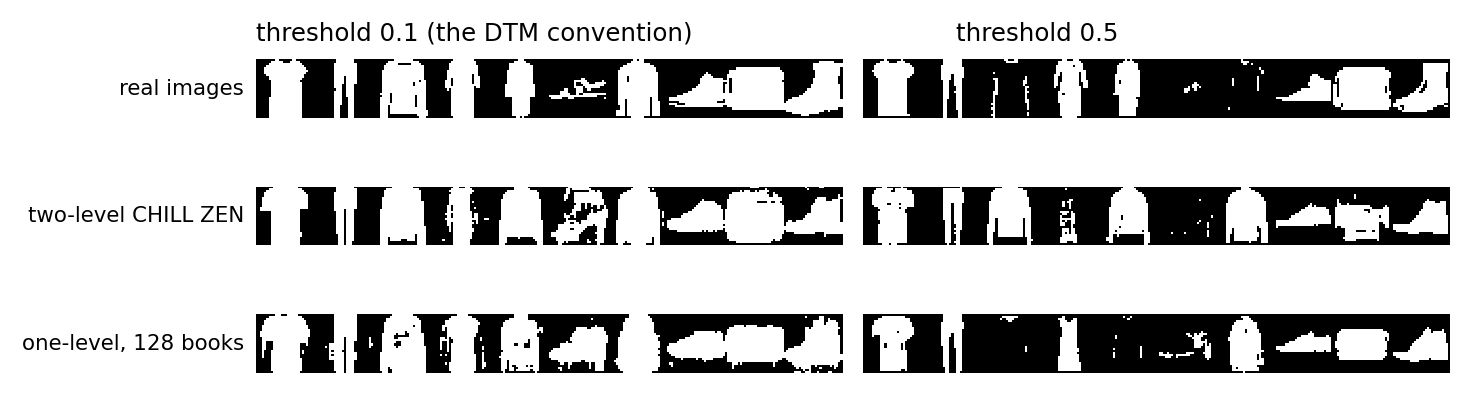
\includegraphics[width=\textwidth]{figures/fig-binarization.png}
\caption{\textbf{The binarization threshold changes every image, and
it is not a model choice.} The same renders, one sample per class,
thresholded at the replication's 0.1 (left) and at
the midpoint (right). Real Fashion-MNIST scored against their own
reference gives FID 0.000039 at 0.1 and 29.75 at 0.5, so the
convention alone spans more than the gap between any two systems in
Table~\ref{tab:headtohead}.}
\label{fig:binarization}
\end{figure*}

\begin{figure*}
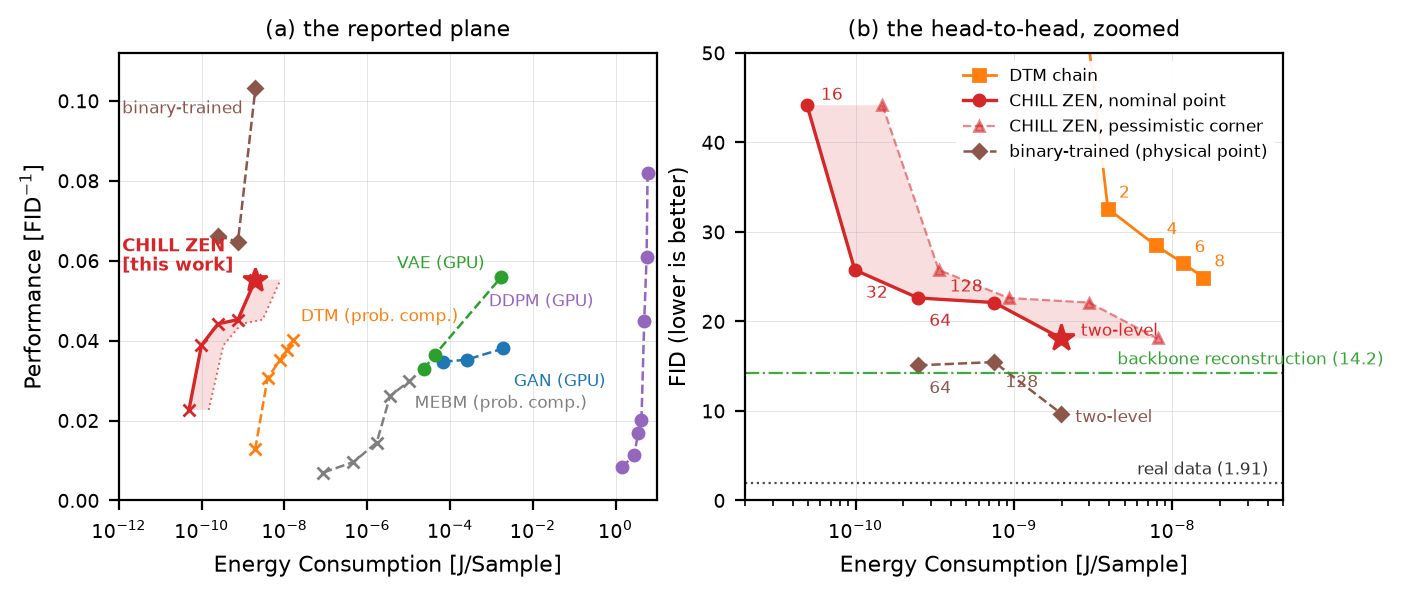
\includegraphics[width=\textwidth]{figures/fig-energy.png}
\caption{\textbf{CHILL ZEN's performance versus energy.}
CHILL ZEN FIDs use the replication protocol of
Table~\ref{tab:protocol}; the other series are published values
whose scoring path we could not verify. The CHILL ZEN
frontier spans one-level systems of 16, 32, 64, and 128 books and the
two-level system (star) at the nominal point of the energy model; the
shaded band extends each point to the model's pessimistic corner
(Appendix~\ref{app:energy}). The binary-trained arms (diamonds) are
plotted at their computed energies. (a) The axes of Fig.~1 of
Ref.~\cite{jelincic2025dtm}, with their five reported series
re-plotted from their data. (b) The same frontier against the DTM
chain alone, drawn as FID so the margin is readable, with the backbone
reconstruction and real-data references. Each CHILL ZEN point is at its own
best comparator level; the two-level system and the 128- and 64-book
one-level systems clear the DTM chain, and the 32- and 16-book
systems do not. The energy values for this work are
estimates from the model of Appendix~\ref{app:energy}.}
\label{fig:energy}
\end{figure*}


\section{Limitations}\label{sec:limitations}

\begin{enumerate}
\item All results are emulator results with bit-exact lane semantics.
    Energy numbers are modeled from a stated
  geometry, not measured, and are reported with their sensitivities for
  that reason. Sending read addresses to the arrays at logic voltage dominates energy
  use. This cost depends on the peripheral transistor pitch and select
  supply. In the pessimistic scenario, the DTM's estimated energy is
  about twice CHILL ZEN's. These scenarios do not bound omitted circuit energy. The model
  covers address delivery, read, and readout energy per image and not
  die area, leakage beyond the bound of Appendix~\ref{app:energy}, or
  the one-time energy of programming the roughly $5.7\times10^{7}$
  memristors the banks require.
\item\label{lim:sneak} Without selectors, the selected symbol contributes only 44\% of the
  nominal crossbar's conductance during a read or feedback pulse. Its
  six row and column neighbors contribute 48\% (Sec.~\ref{app:sneak}). Every
  result of this paper is at the emulator's ideal fidelity, where a
  read returns the selected pair alone; the effect of the sneak share
  on teaching, address resolution, and write disturb has not been
  measured. The $16 \times 1$ selector column of Table~\ref{tab:sneak}
  has no sneak path and is the geometry we would build.
\item The comparator is a model; no circuit has been designed. Its noise is one flat
  term set per read, its offset is assumed trimmed per lane to below a
  tenth of the read voltage at each bias setting, and
  its energy is one estimated constant, with the readout circuit's
  alternatives in Table~\ref{tab:readout}. The operating points of
  Sec.~\ref{sec:comparator} state what a comparator must supply; they
  do not show a circuit that supplies it. The emulator's device
  constants are placeholders pending measurement. The thermal term needs no assumed device constant: at the
  settling-limited pulse, it follows kT/C. The model averages noise over
  the pulse, while a strobed comparator samples it at one instant.
  Sampling raises the lane's thermal noise by about a factor of 1.6
  without changing the conclusions. Only the flicker term requires a device-specific noise constant. It
  contributes 5--70\% of the lane's noise variance; the lane itself
  contributes only a few percent of the draw's variance. Extending the
  model from its 1\,$\mu$s reference pulse to nanosecond pulses assumes
  the $1/f$ noise band reaches those frequencies.
\item The quality bar of Sec.~\ref{sec:results} is a pixel-critic
  agreement score, not FID, because Ref.~\cite{jelincic2025dtm}
  establishes no grayscale reference. The end-to-end critic score exceeds both the reconstruction score and
  the real-image reference by less than its variation across seeds. This
  measures label agreement. Beyond the tests in Sec.~\ref{sec:gap}, we
  have not identified which features of the generated distribution
  affect the score. Contrast still exceeds the alarm threshold:
  std-ratio 1.14 versus 1.10.
\item Our systems are fit on a 68\,000-image split of the full
  70\,000-image dataset, while the reference statistics of
  Sec.~\ref{sec:headtohead} are over the 60\,000-image train split
  that Ref.~\cite{jelincic2025dtm} trains on; the training sets are
  neither identical nor the same size.
\item The scores are validation numbers, not held-out test numbers:
  the evaluation partition was used for epoch and hyperparameter
  selection, and each row of Table~\ref{tab:headtohead} is reported
  at the comparator level that gave its best FID. There is no
  gradient-trained baseline on this code and connectivity, so the
  paper does not claim the local rule outperforms gradient training.
  Conditioning is label-clamped; the unconditional mode of
  Sec.~\ref{sec:headtohead} draws the class from the prior rather
  than learning it.
\end{enumerate}


\section{Conclusion}\label{sec:conclusion}

CHILL ZEN combines a host-fitted additive code with locally taught
lane banks and a fixed generation procedure. The emulator generates
without waiting for an equilibrium distribution, using about 3600
noisy lane reads per image. Pooling leaves too little device noise
at the assumed read voltage, so the comparator must supply most of
the draw variance. On binarized Fashion-MNIST the two-level system
scores FID 18.09, or 9.69 when trained directly on binary data,
against the eight-step DTM's published 24.90. The chain's estimated energy is 7.9 times CHILL ZEN's nominal estimate.
The selector-column design also has a lower energy estimate than the
chain and eliminates the nominal array's sneak paths. These comparisons rest on the stated
scoring protocol and circuit assumptions. The architecture saves energy mainly by reducing sampling work: it
generates each code in a fixed sequence of reads with no equilibrium
mixing phase.

\appendix

\section{List of acronyms}\label{app:acronyms}

\begin{table}[h]
\caption{Acronyms used throughout this work.\label{tab:acronyms}}
\begin{ruledtabular}
\begin{tabular}{lp{5.8cm}}
Acronym & Meaning \\
\colrule
AAT & Activation Address Tuple \\
AHaH & Anti-Hebbian and Hebbian \\
AQ & Additive Quantization \\
AR & Autoregressive \\
CHILL ZEN & Comparator-Heated In-memory Lane
  Learning with Zero-Ended Noise \\
DTCA & Denoising Thermodynamic Computer Architecture \\
DTM & Denoising Thermodynamic Model \\
EBM & Energy-Based Model \\
FID & Fr\'echet Inception Distance \\
GAN & Generative Adversarial Network \\
GPU & Graphics Processing Unit \\
MEBM & Monolithic Energy-Based Model \\
RNG & Random-Number Generator \\
VAE & Variational Autoencoder \\
WTA & Winner-Take-All \\
\end{tabular}
\end{ruledtabular}
\end{table}



\section{The energy model}\label{app:energy}

The energy figures of Sec.~\ref{sec:energy} come from the model below,
a physical estimate from a stated geometry; the script that computes it
is named in Sec.~\ref{app:code}.

\subsection{Scope}\label{app:scope}

The model counts three terms per generated image: the delivery of
each read's address to the memristor arrays, the divider reads
themselves, and the per-lane readout. It excludes rail supplies and leakage, estimated in
Sec.~\ref{app:excluded}, and comparator kickback, which remains
unverified. The estimate excludes weight-programming energy and die area, with no
bound on either. This follows Ref.~\cite{jelincic2025dtm}, which omits
its own weight programming and reports only per-sample energy. The
basis of comparison is stated in Sec.~\ref{app:basis}.

\subsection{Geometry}\label{app:geometry}

The lane is the neural lane of Ref.~\cite{knowm2026blog}, Chapter~4. Its element is the \emph{unit crossbar}, a small memristor crossbar. Row
and column multiplexers select one device between source and drain
lines. With no selector transistor at each memristor, floating
unselected rows and columns allow current through other devices. A synapse
is a pair of unit crossbars, the $a$-side between rail $V_a$ and the
output node and the $b$-side between the node and rail $V_b$. A lane is
$K$ such pairs, one per address space, with every pair's midpoint tied
to one output line $V_y$. Selection is the AAT: one address per space,
broadcast to every lane of a bank.

The array is an integrated crossbar with a 20\,nm via at each crossing
and the memristor in the via, on a 50\,nm pitch. Each space of the
deployed system has 16 symbols, so the nominal unit crossbar is the
smallest that holds them, a $4 \times 4$ array 0.20\,$\mu$m on a side
with two 4:1 pass-transistor multiplexers and $2 + 2$ address bits. A
$16 \times 16$ array is carried as a sensitivity.

Three consequences of that layout fix the capacitances
(Fig.~\ref{fig:app-geometry}):

\begin{enumerate}
\item \emph{The select lines of a space run across the bank.} Every lane
  of a bank reads the same context, so the four row-select and four
  column-select lines of space $k$ cross all $L$ lanes. The $a$- and
  $b$-side multiplexers of a pair take the same address, so one row line
  and one column line serve both, each driving two pass gates per lane.
  Asserting a symbol charges two lines per (space, lane).
\item \emph{The multiplexers set the lane pitch, not the array.} Along a
  select line one lane is one unit crossbar wide: the 0.20\,$\mu$m array
  plus one stack of four pass transistors at the contacted transistor
  pitch $t$, so $p = 4d + 4t$ with $d$ the crossbar pitch. At $t =
  0.20\,\mu$m (a 28--40\,nm-class periphery) $p = 1.00\,\mu$m; at $t =
  0.06\,\mu$m (a 7\,nm-class periphery) $p = 0.44\,\mu$m. Total energy is only weakly sensitive to via and crossbar pitch:
  doubling $d$ to 100\,nm changes it by less than 5\%.
\item \emph{The $V_y$ node is $2K$ lane pitches long and carries $8K$
  multiplexer drains.} The $a$ and $b$ arrays of a pair and the $K$
  spaces all stack along $V_y$. Its capacitance is
  $C_{\mathrm{node}} = K\,(2 p\, c_w + 8\, C_d)$ with $c_w$ the wire
  capacitance per length and $C_d$ the drain capacitance of an off pass
  transistor.
\end{enumerate}

\begin{figure}
\centering
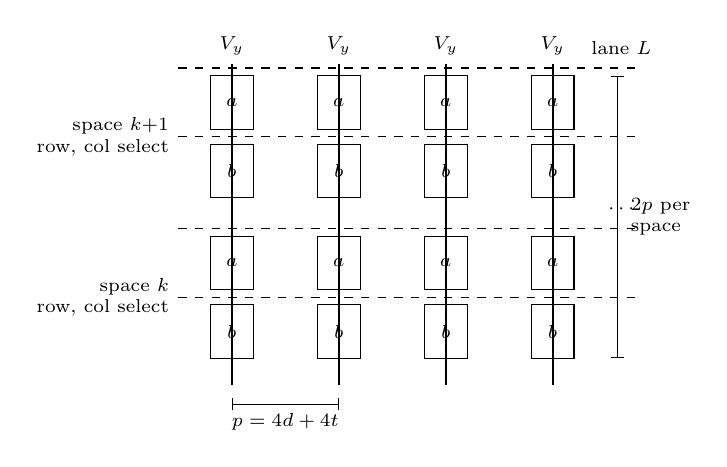
\begin{tikzpicture}[font=\scriptsize, x=1cm, y=1cm, scale=0.97, transform shape]
  % lanes: vertical Vy lines
  \foreach \i in {0,1,2,3} {
    \draw[thick] (\i*1.4, -0.3) -- (\i*1.4, 3.9);
    \node[above] at (\i*1.4, 3.9) {$V_y$};
  }
  \node[above] at (4.2+0.9, 3.9) {lane $L$};
  \node at (4.2+0.9, 2.0) {$\cdots$};
  % unit crossbar pairs at spaces k and k+1
  \foreach \i in {0,1,2,3} {
    \foreach \k/\yy in {0/0, 1/2.1} {
      \draw (\i*1.4-0.28, \yy+0.05) rectangle (\i*1.4+0.28, \yy+0.75);
      \node at (\i*1.4, \yy+0.40) {$b$};
      \draw (\i*1.4-0.28, \yy+0.95) rectangle (\i*1.4+0.28, \yy+1.65);
      \node at (\i*1.4, \yy+1.30) {$a$};
    }
  }
  % select lines (row + column) for space k and k+1, crossing all lanes
  \foreach \k/\yy in {0/0, 1/2.1} {
    \draw[dashed] (-0.7, \yy+0.85) -- (5.3, \yy+0.85);
    \draw[dashed] (-0.7, \yy+1.75) -- (5.3, \yy+1.75);
  }
  \node[left, align=right] at (-0.7, 0.85) {space $k$\\row, col select};
  \node[left, align=right] at (-0.7, 2.95) {space $k{+}1$\\row, col select};
  % lane pitch p
  \draw[{Bar}-{Bar}] (0, -0.55) -- (1.4, -0.55);
  \node[below] at (0.7, -0.55) {$p = 4d + 4t$};
  % Vy length 2Kp
  \draw[{Bar}-{Bar}] (5.05, 0.05) -- (5.05, 3.75);
  \node[right, align=left] at (5.1, 1.9) {$2p$ per\\space};
\end{tikzpicture}
\caption{The geometry the model assumes. Each box is one unit
crossbar; a pair ($a$ over $b$) is one synapse, and the pairs of a lane
stack along its output line $V_y$. The dashed lines are the row- and
column-select lines of a space, shared by every lane of the bank. A read
charges the two select lines of every asserted space across all $L$ lanes
(term $E_{\mathrm{sel}}$) and settles each lane's $V_y$ node through the
selected devices (term $E_{\mathrm{read}}$). The lane pitch $p$ along a
select line is the $4 \times 4$ array plus one multiplexer stack of four
pass transistors; the node is $2p$ long per space.}
\label{fig:app-geometry}
\end{figure}

\begin{table}
\caption{Derived dimensions and capacitances, from the constants of
Table~\ref{tab:app-constants}.\label{tab:app-derived}}
\footnotesize
\begin{ruledtabular}
\begin{tabular}{lcc}
quantity & nominal & 7\,nm-class \\
\colrule
transistor pitch $t$ & 0.20\,$\mu$m & 0.06\,$\mu$m \\
lane pitch $p = 4d + 4t$ & 1.00\,$\mu$m & 0.44\,$\mu$m \\
$C_{\mathrm{seg}} = 2C_g + p\,c_w$ per lane & 0.80\,fF & 0.29\,fF \\
$C_{\mathrm{node}}$, backbone and patch lanes ($K = 134$) & 161\,fF & 131\,fF \\
$C_{\mathrm{node}}$, joint and decode lanes ($K = 232$) & 278\,fF & 226\,fF \\
\end{tabular}
\end{ruledtabular}
\end{table}

\subsection{Operation count}\label{app:census}

The operation count of the deployed two-level system is exact, taken
from the banks' lane and space counts. The generation of one image reads
five banks (Table~\ref{tab:app-census}). Two counts enter the model per
bank: the number of (space, lane) assertions, $L K$, which is what the
select lines must deliver, and the number of lane reads, which is what
the nodes and comparators must resolve. The backbone draw and patch draw
are hot reads at 10\,mV; the sweeps and the decode are cold reads at
50\,mV.

The backbone draw is 128 sequential steps, each reading a fresh group of
16 lanes with one more space asserted. Select lines span the bank, so selecting space $k$ for group $k$ also
activates it in groups that have already read. Only 142\,336 of the $g$
bank's 276\,576 select assertions contribute to a read. Segmenting the lines per group would save 48\% of
the $g$ bank's $E_{\mathrm{sel}}$, 7.5\% of the total
$E_{\mathrm{sel}}$, with a driver per group per space; the
model does not include it.

\begin{table*}
\caption{The per-image operation count and each bank's contribution at the
nominal point. Lanes: $g$ bank $(1 + 128) \times 16$, $r$ bank $128
\times 16$, patch $98 \times 16$, joint $226 \times 16$, decode 784.
\label{tab:app-census}}
\begin{ruledtabular}
\begin{tabular}{lrrrrrr}
bank & $L$ & $K$ & $LK$ & reads & $V_{\mathrm{read}}$ &
  $E_{\mathrm{sel}}$ (J) \\
\colrule
backbone draw ($g$) & 2064 & 134 & 276\,576 & 2048 & 10\,mV & $2.8\times10^{-10}$ \\
backbone sweep ($r$) & 2048 & 134 & 274\,432 & 2048 & 50\,mV & $2.8\times10^{-10}$ \\
patch draw & 1568 & 134 & 210\,112 & 1568 & 10\,mV & $2.2\times10^{-10}$ \\
joint sweep & 3616 & 232 & 838\,912 & 3616 & 50\,mV & $8.6\times10^{-10}$ \\
decode & 784 & 232 & 181\,888 & 784 & 50\,mV & $1.9\times10^{-10}$ \\
\colrule
total & & & 1\,781\,920 & 10\,064 & & $1.8\times10^{-9}$ \\
\end{tabular}
\end{ruledtabular}
\end{table*}

\subsection{Energy terms}\label{app:terms}

Per image,
\begin{equation}
E = E_{\mathrm{sel}} + E_{\mathrm{read}} + E_{\mathrm{readout}} +
    E_{\mathrm{rail}} .
\label{eq:app-total}
\end{equation}

\emph{Address delivery.} For each bank, each space asserted per image
charges one row line and one column line across every lane of the bank.
A line charged once and discharged once per image dissipates $C V^2$:
\begin{equation}
E_{\mathrm{sel}} = \sum_{\mathrm{banks}} L\, K \cdot 2\,
  C_{\mathrm{seg}}\, V_{\mathrm{sel}}^2 ,
\qquad C_{\mathrm{seg}} = 2 C_g + p\, c_w .
\label{eq:app-sel}
\end{equation}
This is the term Ref.~\cite{jelincic2025dtm} calls $E_{\mathrm{comm}}$,
the charging of the parasitic capacitance of the wires that carry a
cell's state to its neighbors, and reports as about half of its budget.

\emph{The divider read.} A lane read settles its $V_y$ node through the
selected devices and pass gates. With the pulse width set by settling,
$t = 5RC = 5\,C_{\mathrm{node}} / G_\Sigma$,
\begin{equation}
E_{\mathrm{read}} = \sum_{\mathrm{reads}} V_{\mathrm{read}}^2\, G_\Sigma\, t
  = \sum_{\mathrm{reads}} 5\, C_{\mathrm{node}}\, V_{\mathrm{read}}^2 .
\label{eq:app-read}
\end{equation}
The pooled conductance cancels; the factor 5 is for rails at $\pm V$
about the node and a balanced pool, so that each side settles through
$V$. Changes that affect only conductance alter settling time but leave read
energy unchanged. These include device conductance range, size, write
compliance, and sneak conductance in a crossbar with floating lines.
Sneak conductance does change what the node reads: in a $4 \times 4$
array with floating unselected lines the selected device is $7/16$ of
the conductance the node sees. Sec.~\ref{app:sneak} derives that and
the energy of each way out, and Limitation~\ref{lim:sneak} states what
follows for the results.

Equation~(\ref{eq:app-read}) also qualifies the thermodynamic identity
of Sec.~\ref{sec:energy}, Eq.~(\ref{eq:ethermal}). That identity, $E\,\sigma^2 = 2\kB T$, assumes the read
integrates the node over the full pulse. A comparator that samples the
node sees its $\kB T / C$ noise, $\sigma^2 = \kB T / (C_{\mathrm{node}}
V^2)$, and with $E = 5 C_{\mathrm{node}} V^2$ the realized product is
$5 \kB T$. The identity remains a floor on the lane's own contribution
to a hot read's noise; it does not enter the accounting.

\emph{Readout.} One comparator per lane resolves the read against the
group's shared falling reference (Sec.~\ref{sec:routines}). The model assumes a continuous-time comparator with a preamplifier and
latch drawing 200\,nA from 0.8\,V for 62.5\,ns. This gives 10\,fJ per
lane read for bias current; the model assigns no separate energy to the
decision. The lane buffer of the readout circuit of
Ref.~\cite{knowm2026blog}, ``The RankCut recoder in hardware,'' a
follower biased at 100\,nA for the same window, dissipates 5\,fJ:
\begin{equation}
E_{\mathrm{readout}} = N_{\mathrm{reads}} \times 15\,\mathrm{fJ} .
\label{eq:app-readout}
\end{equation}
The continuous-time comparator triggers when the reference crosses the
lane voltage. This gives one noise sample per lane, as in the emulator,
if the reference crosses the comparator's $\pm 3\sigma$ band within one
noise correlation time. The required slope is at least $6 v_n \cdot 2\pi
B$. At $v_n = 2$\,mV and $B = 500$\,MHz, this is 38\,mV/ns, enough to
sweep the 20\,mV range in about 0.5\,ns. Reducing preamplifier bias increases noise (Sec.~\ref{sec:comparator}):
the input-referred thermal noise variance is $4 \kB T \gamma B / g_m$,
where $g_m = I / (n V_T)$. At fixed bandwidth-time product $BT$, the
energy per read for rms noise $v_n$ is $4 \kB T \gamma\, n V_T V_{dd}\,
(BT) / v_n^2$. With $\gamma = 1$, $n V_T = 35$\,mV, and an illustrative
$BT = 3$, a 2\,mV hot read uses 0.35\,fJ. Lower noise requires more
energy: 1.4\,fJ at 1\,mV (code 45), 15\,fJ at 300\,$\mu$V (code 10), and
139\,fJ at 100\,$\mu$V (code 0). These noise-energy examples use $BT=3$, whereas 500\,MHz over the
model's 62.5\,ns window gives $BT=31.25$ and energies 10.4 times
larger. They therefore do not establish that the modeled comparator
meets both the hot-read ramp condition and the cold-noise requirement.
The cold-noise control measures grayscale sensitivity, not circuit
feasibility or FID at that circuit's noise level.
Table~\ref{tab:readout} compares the alternatives, printed by
\texttt{experiments/38\_readout\_options.py}. A clocked comparator with a falling reference returns every lane's
rank, with one strobe and fresh noise sample per reference step.
A clocked pairwise tournament returns only the winner, which is all
generation uses, at one decision per lane. A continuous-time comparator
returns both winner and rank; its standing bias energy depends on the
required noise level.

\begin{table*}
\caption{Five readout circuits on the deployed census with the
nominal constants; every row is printed by
\texttt{experiments/38\_readout\_options.py}. Clocked decisions dissipate
10\,fJ each; continuous-time rows are bias times supply times the
62.5\,ns window; every row carries the 5\,fJ lane buffer. The noise
column says how many independent comparator noise samples a lane's
decision passes through: the emulator computes one.\label{tab:readout}}
\footnotesize
\begin{ruledtabular}
\begin{tabular}{>{\raggedright\arraybackslash}p{4.6cm}>{\raggedright\arraybackslash}p{2.6cm}>{\raggedright\arraybackslash}p{3.6cm}ccc}
readout circuit & returns & noise samples per lane read & per lane read
  & readout share & ratio \\
\colrule
continuous-time, 200\,nA for 62.5\,ns, as modeled & winner and rank &
  one, when the reference falls faster than the noise correlation time
  & 15\,fJ & 8\% & $7.9\times$ less \\
continuous-time, 1\,$\mu$A for 62.5\,ns & winner and rank & one, at
  $\sqrt{5}$ lower noise & 55\,fJ & 23\% & $6.5\times$ less \\
clocked, binary search on the winner, 5 strobes & winner only & five,
  the first crossing decides & 55\,fJ & 23\% & $6.5\times$ less \\
clocked, full ramp, 16 strobes & winner and 4-bit rank & sixteen, the
  first crossing decides & 165\,fJ & 47\% & $4.5\times$ less \\
clocked tournament, 15 pairwise decisions per group & winner only & one
  per comparison, on lane differences & 14\,fJ & 7\% & $7.9\times$ less \\
\end{tabular}
\end{ruledtabular}
\end{table*}

\emph{Rails.} The rails $V_a$ and $V_b$ apply the instruction's voltage
during the read pulse and return to node potential between reads. Each
lane therefore conducts only during its own read. Holding the rails
active throughout generation would keep every selected device in the
bank conducting. Charging the rails per read is bounded in
Sec.~\ref{app:excluded} and carried as zero.

\subsection{Sneak paths and the ways out}\label{app:sneak}

The nominal $4 \times 4$ array has no selector and floats its
unselected lines. With every device at a common conductance $G$ the
sneak network puts $1.29G$ in parallel with the selected device, so
the selected device is $7/16$ of what the node sees: a read is 44\%
the selected symbol, 48\% its six row and column neighbors, and 8\%
the other nine, and a feedback pulse divides the same way. At a
$16 \times 16$ array the selected share is 12\%. The nodal solve is
\texttt{experiments/36\_sneak\_paths.py}.

Table~\ref{tab:sneak} compares three ways out. Holding the node-side
unselected lines at ground makes the read exact but shunts the node
with $2.25G$ per side, a gain loss of about three that the read
voltage must make up. Holding them at a replica of $V_y$ is exact but
needs a per-lane buffer whose bias the model cannot estimate. A $16 \times 1$ selector column uses one 1-of-16 multiplexer on the rail
side and none on the node side. It eliminates sneak paths and charges
one select line per assertion instead of two, using less energy than the
$4 \times 4$ array. It requires twice as many select lines and 2.5 times
as many leakage paths. Leakage remains negligible only because the rails
pulse during each read (Sec.~\ref{app:excluded}).

\begin{table*}[t!]
\caption{The energy of each way out of the sneak paths, by the
model of Appendix~\ref{app:energy} on the deployed census with the
nominal constants; every row is printed by
\texttt{experiments/36\_sneak\_paths.py}. The read column is for a
$4 \times 4$ array with every device at a common conductance $G$. The
two selector-column rows differ only in whether the sixteen pass
gates sit beside the array or stack along $V_y$.\label{tab:sneak}}
\footnotesize
\begin{ruledtabular}
\begin{tabular}{>{\raggedright\arraybackslash}p{3.4cm}>{\raggedright\arraybackslash}p{4.0cm}>{\raggedright\arraybackslash}p{3.9cm}ccc}
geometry & what the node reads & added circuitry & $E_{\mathrm{sel}}$ (J) &
  total (J) & ratio \\
\colrule
$4 \times 4$, floating lines, as modeled & 44\% the selected symbol,
  48\% its six row and column neighbours, 8\% the other nine & none &
  $1.8\times10^{-9}$ & $2.0\times10^{-9}$ & $7.9\times$ less \\
$4 \times 4$, node-side lines at fixed ground & the selected pair at a
  gain of 0.31; the hot read rises to 32.5\,mV to restore 10\,mV at the
  comparator & a pull-down gate per node-side line per lane, on a
  complement select line & $2.7\times10^{-9}$ & $3.0\times10^{-9}$ &
  $5.2\times$ less \\
$4 \times 4$, node-side lines track $V_y$ & the selected pair & the
  same pull-downs, to a per-lane replica of $V_y$; the buffer that
  drives it is unpriced & $2.7\times10^{-9}$ & $3.0\times10^{-9}$ &
  $5.2\times$ less \\
$16 \times 1$ selector column, pass gates beside the array & the
  selected pair & sixteen select lines per space instead of eight; no
  node-side multiplexer & $1.4\times10^{-9}$ & $1.6\times10^{-9}$ &
  $9.9\times$ less \\
$16 \times 1$ selector column, pass gates stacked along $V_y$ & the
  selected pair & the same & $7.4\times10^{-10}$ & $9.1\times10^{-10}$
  & $17.2\times$ less \\
\end{tabular}
\end{ruledtabular}
\end{table*}

\subsection{Constants}\label{app:constants}

Every constant is a stated dimension or a textbook value
(Table~\ref{tab:app-constants}). The model has no fitted parameter.

\begin{table}
\caption{The constants of the model and their sources.
\label{tab:app-constants}}
\footnotesize
\begin{ruledtabular}
\begin{tabular}{lcp{2.9cm}}
constant & value & source \\
\colrule
via diameter & 20\,nm & stated geometry \\
crossbar pitch $d$ & 50\,nm & stated geometry; the total is insensitive to it \\
unit crossbar & $4 \times 4$ & smallest that holds a 16-symbol space; $16 \times 16$ as sensitivity \\
transistor pitch $t$ & 0.20\,$\mu$m & 28--40\,nm-class design rules; 0.06\,$\mu$m for 7\,nm-class \\
pass-gate capacitance $C_g$ & 0.3\,fF & minimum-size device \cite{weste2011cmos}; 0.1\,fF for 7\,nm-class \\
wire capacitance $c_w$ & 0.2\,fF/$\mu$m & minimum-width metal with neighbors \cite{weste2011cmos} \\
off-drain capacitance $C_d$ & 0.1\,fF & same \\
select supply $V_{\mathrm{sel}}$ & 0.8\,V & core supply; 0.5\,V as low-swing sensitivity \\
read voltage, hot / cold & 10 / 50\,mV & the operating point of Sec.~\ref{sec:comparator} \\
comparator + buffer & 15\,fJ & continuous-time comparator at 200\,nA and a 100\,nA buffer, both at 0.8\,V over the 62.5\,ns window; Table~\ref{tab:readout} for the alternatives; 45\,fJ as sensitivity \\
DTM chain & $1.57 \times 10^{-8}$\,J & Ref.~\cite{jelincic2025dtm}, Fig.~1, deepest chain, decoded from the figure; their text's $1.6\,T$\,nJ gives $1.28 \times 10^{-8}$ \\
\end{tabular}
\end{ruledtabular}
\end{table}

\subsection{Results}\label{app:results}

Table~\ref{tab:app-results} gives the total at the nominal point and at
the stated sensitivities. Changing one nominal parameter at a time gives these DTM-to-CHILL ZEN
energy ratios: 6.4 with separate $a$- and $b$-side select lines; 4.6
with $16 \times 16$ arrays; 6.8 with 45\,fJ readout; 5.0 with
0.3\,fF/$\mu$m wire and 0.5\,fF gates; 7.5 with 100\,nm crossbar pitch;
and 6.6 with 0.4\,$\mu$m transistor pitch. $E_{\mathrm{read}}$ never exceeds 4\% of the total at
any point in the table.

\begin{table*}
\caption{The energy terms at each operating point. Every row is
printed by the script of
Sec.~\ref{app:code}.\label{tab:app-results}}
\begin{ruledtabular}
\begin{tabular}{lcccc}
operating point & $E_{\mathrm{sel}}$ & $E_{\mathrm{read}}$ &
  total (J) & ratio \\
\colrule
nominal & $1.8\times10^{-9}$ & $2.0\times10^{-11}$ &
  $2.0\times10^{-9}$ & $7.9\times$ less \\
low-swing select, 0.5\,V & $7.1\times10^{-10}$ & $2.0\times10^{-11}$ &
  $8.8\times10^{-10}$ & $17.7\times$ less \\
7\,nm-class periphery & $6.6\times10^{-10}$ & $1.6\times10^{-11}$ &
  $8.2\times10^{-10}$ & $19.0\times$ less \\
7\,nm-class, 0.5\,V & $2.6\times10^{-10}$ & $1.6\times10^{-11}$ &
  $4.2\times10^{-10}$ & $37.0\times$ less \\
pessimistic corner\footnote{$16 \times 16$ arrays, separate $a$- and
  $b$-side select lines, 1.0\,V.} & $7.8\times10^{-9}$ &
  $7.9\times10^{-11}$ & $8.1\times10^{-9}$ & $1.9\times$ less \\
\end{tabular}
\end{ruledtabular}
\end{table*}

Ref.~\cite{jelincic2025dtm} estimates cell energy from foundry models
for an unnamed advanced process node. The 7\,nm-class rows illustrate
how such a process could affect our design. Our energy claim uses the
nominal row.

\subsection{Bounds on the excluded terms}\label{app:excluded}

\emph{Rails.} The rails run along each lane beside $V_y$; their wire
capacitance across all 10\,080 lanes is 1.4\,nF. Asserting a bank's
rails once per read step at that read's voltage, 128 steps for the
$g$ bank and one for each of the others, dissipates $5 \times
10^{-12}$\,J per image, 0.3\% of the nominal total.

\emph{Leakage.} No transistor sits at a memristor, and the select lines
have no DC path. The DC paths are the off pass gates of both
multiplexers of a pair while its rail is asserted: $2 \times 2 \times
3 = 12$ per space, $2.1 \times 10^{7}$ over the census, at about 5\,pA
each with at most the read voltage across them. Because the rails are
asserted per read, those gates leak only during the read pulses: for
pulses of 10\,ns per step that is $2.5 \times 10^{-13}$\,J per image,
below $10^{-4}$ of the total. Had the rails been held across an assumed
30\,$\mu$s image at 50\,mV, the same gates would leak $1.6 \times
10^{-10}$\,J, 8\% of the total, which is one reason the rails are
pulsed. The image time itself depends on the device's conductance,
which the model does not need and the paper does not claim.

\emph{Comparator kickback.} An illustrative 0.5\,fC input charge
would move a 131\,fF node by about 4\,mV, but the first backbone
read has only about 12\,fF including comparator input capacitance,
which gives about 42\,mV. A fixed trim cannot be assumed to cancel
state-dependent kickback across these loads. Kickback is absent from
the emulator and remains a readout-design requirement, not a verified
negligible term.

\emph{Read disturb.} The cold read at 50\,mV is two times below the
erase threshold and five times below the 0.25\,V write threshold; the
hot read at 10\,mV is ten and twenty-five times below.

\subsection{Basis of comparison}\label{app:basis}

Ref.~\cite{jelincic2025dtm} models its per-sample energy as $E = T
K_{\mathrm{mix}} L^2 E_{\mathrm{cell}}$ with $E_{\mathrm{cell}} =
E_{\mathrm{rng}} + E_{\mathrm{bias}} + E_{\mathrm{comm}} +
E_{\mathrm{clock}} \approx 2$\,fJ per conditional update, the RNG term
measured on a test chip and the rest from foundry models at a node the
paper does not name. It excludes weight programming, host
communication, and die area. The present model counts the same kinds of
term (wire charging, per-cell readout, the analog operation itself) for
the same unit of work (one generated image), excludes the same things,
and states its process class explicitly. The voltage assumptions favor the DTM: it signals neighbors at $4 V_T
\approx 100$\,mV and clocks at $5 V_T$, while our select lines use the
0.8\,V core supply. The 0.5\,V row shows the savings from reducing our
select voltage. The chain energy used throughout,
$1.57\times10^{-8}$\,J, is the deepest point of their Fig.~1 decoded
from the vector figure ($1.961\,T$\,nJ at $T = 8$); their text puts
the same model at ``around $1.6\,T$\,nJ,'' which is
$1.28\times10^{-8}$\,J and makes the nominal ratio 6.4 rather than
7.9. If lane decoding (Sec.~\ref{sec:energy}) is unavailable, a digital $784
\times 226$ matrix-vector product adds 1.8--8.9\,nJ to the 2.0\,nJ
estimate, assuming 10--50\,fJ per 8-bit multiply-accumulate. The two accountings are
therefore comparable in kind, and both
are estimates: theirs extrapolated from one fabricated circuit, ours
from a stated geometry.

\subsection{Code}\label{app:code}

The model is one function of the operation count and the constants of
Table~\ref{tab:app-constants}. It is computed by
\texttt{chill\_zen/energy\_geom.py} in the repository
\url{https://github.com/knowm/CHILL-ZEN}, and every row of
Table~\ref{tab:app-results} is printed by
\texttt{experiments/12\_energy\_model.py} from the banks' own lane and
space counts. The one-level frontier of Fig.~\ref{fig:energy} and the binary-trained
arms are computed by \texttt{experiments/13\_energy\_frontier.py} and
\texttt{experiments/22\_binary\_energy.py} from their own operation counts with
the same constants. \texttt{NUMBERS.md} in the repository lists each
number of this appendix beside the script that produces it.

\section*{Declarations}

\subsection*{Data and Code Availability}

The companion repository contains the final experimental recipe,
paper source, saved numerical evidence, and a map from reported
quantities to scripts. It is prepared for release at \url{https://github.com/knowm/CHILL-ZEN}, with the
lane emulator at \url{https://github.com/knowm/ktram-neural-core}.
The evaluation of Sec.~\ref{sec:headtohead} imports the released
feature extractor and distance code of Ref.~\cite{dtmreplication} and
scores against its shipped reference statistics; we do not
redistribute them, and the repository records
the commit, the file checksums, and the harness that calls them. The
companion repository is released under the MIT license.

\subsection*{Acknowledgments}

I thank the authors of Ref.~\cite{jelincic2025dtm} for an energy
analysis specific enough to argue with, and the authors of
Ref.~\cite{dtmreplication} for publishing the evaluation code that
made the argument checkable.

Every experiment reported here ran on the CPU of my old Intel iMac while I was walking the dogs, asleep, doing
chores, or attending to other small businesses. I used AI to run the experiments, gather the data, and draft this
paper. I spent many
hours trying to get AI to remove its own slop, to the point where it
might have been faster to write the whole thing myself. Before release the draft went through several rounds of
simulated hostile review, each run with the most capable model
available to me at the time, Claude Fable 5.1 and OpenAI Astra-6. They reviewed the paper, code, logs, and source of
Ref.~\cite{jelincic2025dtm}, then listed gaps, inconsistencies, and
misattributions in order of severity. Each round added corrections and more AI slop, which I removed by hand. 

\subsection*{Competing Interests}

The author is part of Knowm Inc., which has made and sold memristors and
plans to sell products or intellectual property based on technologies
described here. The kT-bit, the
kT-RAM architecture, and its technology stack are the subject of
granted U.S. patents
\cite{nugent2015ktbitpatent,nugent2017ktrampatent,nugent2019stackpatent};
the portfolio is listed at \url{https://knowm.ai/ip/}.

\bibliography{refs}

\end{document}
